\documentclass{cernatsnote}
%\usepackage[colorinlistoftodos]{todonotes}
\usepackage[utf8]{inputenc}
%\usepackage{placeins}
\usepackage{pdfpages,multirow,ragged2e} %
\usepackage{subcaption}
\usepackage{graphicx}
\usepackage{longtable}
\usepackage{booktabs}
\usepackage{float}
\usepackage{tabulary}
\usepackage{tabularray}

\title{Optics commissioning in Run~3}
\author{T.~Persson,  F.~Carlier, A.~Costa~Ojeda, J.~Dilly, H. Garc\'ia Morales, S.~Fartoukh,  V.~Ferrentino, E.~Fol, M.~Hofer, E.J~Høydalsvik, J.~Keintzel, M.~Le~Garrec, E.H.~Maclean, L.~Malina,  F.~Soubelet, R.~Tom\'as, L.~Van Riesen-Haupt and A.~Wegscheider and J. Cardona, 
  %Universidad Nacional de Colombia \\		
%	CERN, CH-1211 Geneva, Switzerland
}
\date{\today}

\begin{document}
\maketitle

\begin{abstract}

\end{abstract}
\\ \\ \\ 

\begingroup
\color{black}
\tableofcontents
\endgroup

\pagebreak

\section{Introduction}

The Run~3 presents a new set of challenges for the optics commissioning. Run~2 was started with a moderate $\beta^*$ of 80~cm and it was then reduced in yearly steps~\cite{ACcom, ewen2019jour}. This gave time to optimize the corrections iteratively as well as focusing on the linear optics in the first 2 years, shifting the focus to the nonlinear IR contributions in the rest of the run. Another challenge is the increase of the range in the operational $\beta^*$ for physics~\cite{run3}, requiring accurate corrections for a larger number of optics. Run~3 optics features the largest telescopic squeeze factor~\cite{ats_stephane} used in operation so far, implying the largest arc $\beta$ functions and the consequent enhancement of arc optics errors.
The Run 3 energy has been increased from 6.5~TeV in Run 2 to 6.8~TeV which could have some consequences for the magnetic field quality.

In 2021 a dedicated beam test took place at injection energy. The results from these measurements are also outlined in this report. 

\section{Local corrections}
\section{Injection}

During Long Shutdown 2 (LS2) it was decided to remove one warm quadrupole on either side of IP7, MQWA.E5, to replace it with shielding~\cite{roderik}.  


\subsection{Linear Corrections}
The beam test week took place in the autumn of 2021 with the intention of testing the LHC after the LS2 to be ready for the full restart in 2022.
The initial measurement of the $\beta$-beat showed significantly higher values than what was measured previously during commissioning. This is shown in Fig.~\ref{fig:initalVs2016} for Beam~1 and Beam~2 respectively.  


\begin{figure}[ht]
\begin{subfigure}{.5\textwidth}
  \centering
  % include first image
  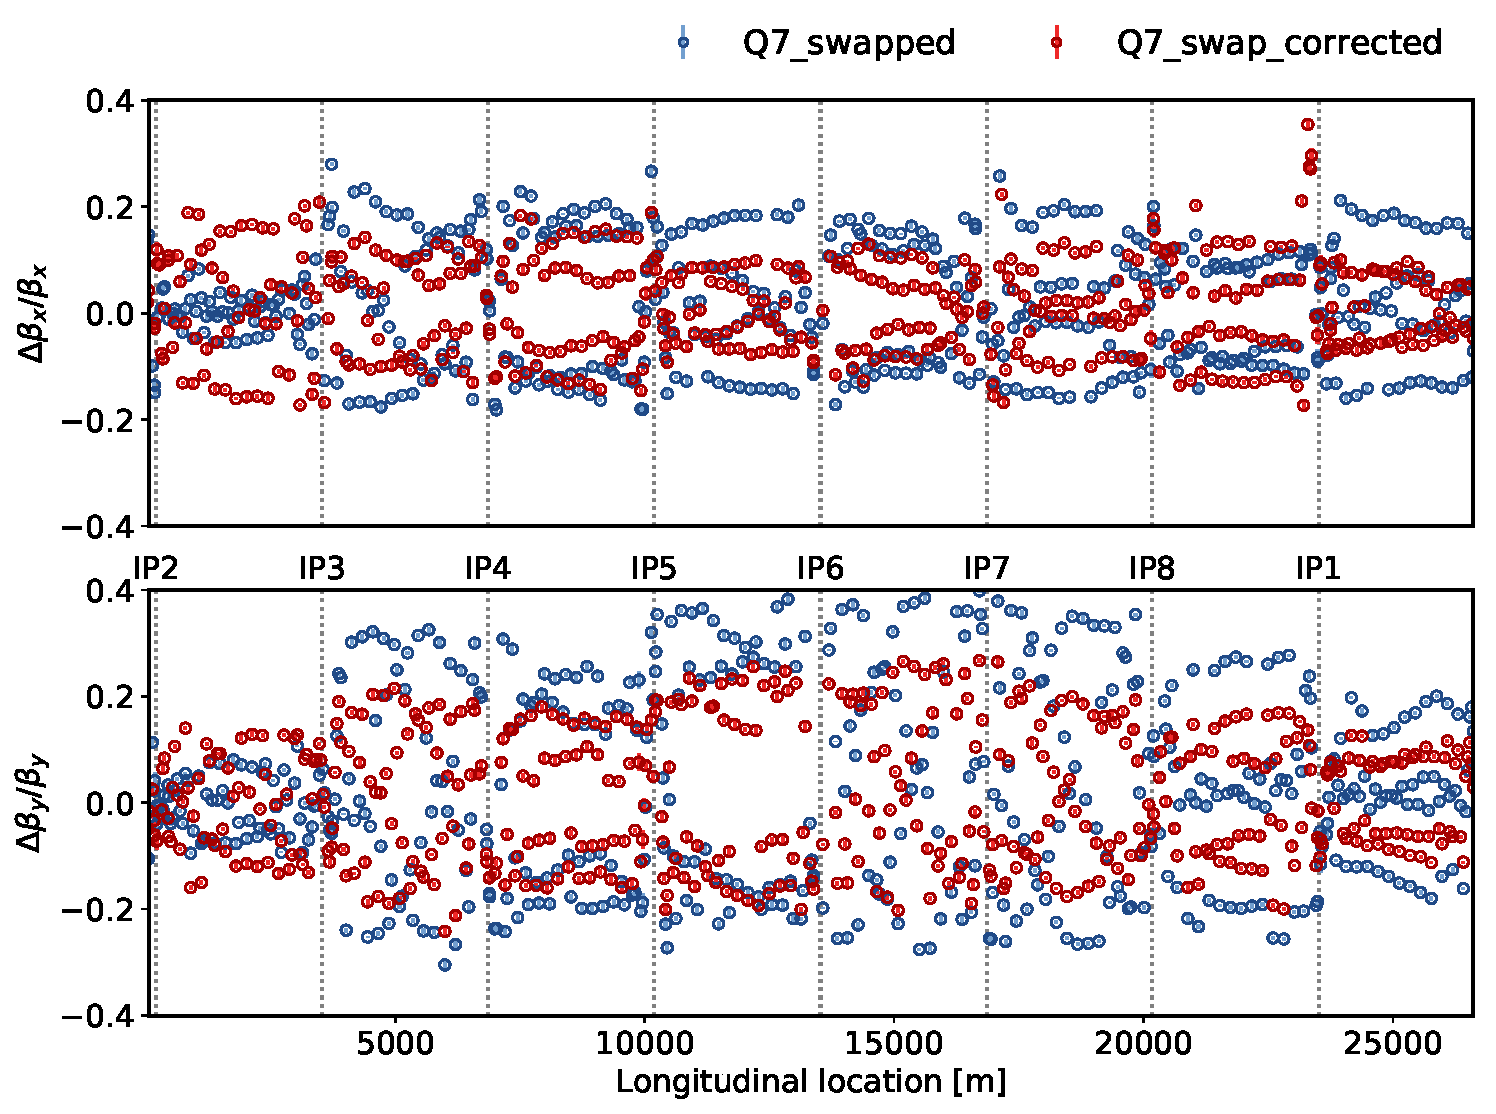
\includegraphics[width=.98\linewidth]{inj_linear/beamtest/beam1/beta_beat_before_after_swap.pdf}  
  \caption{Beam~1}
\end{subfigure}
\begin{subfigure}{.5\textwidth}
  \centering
  % include second image
  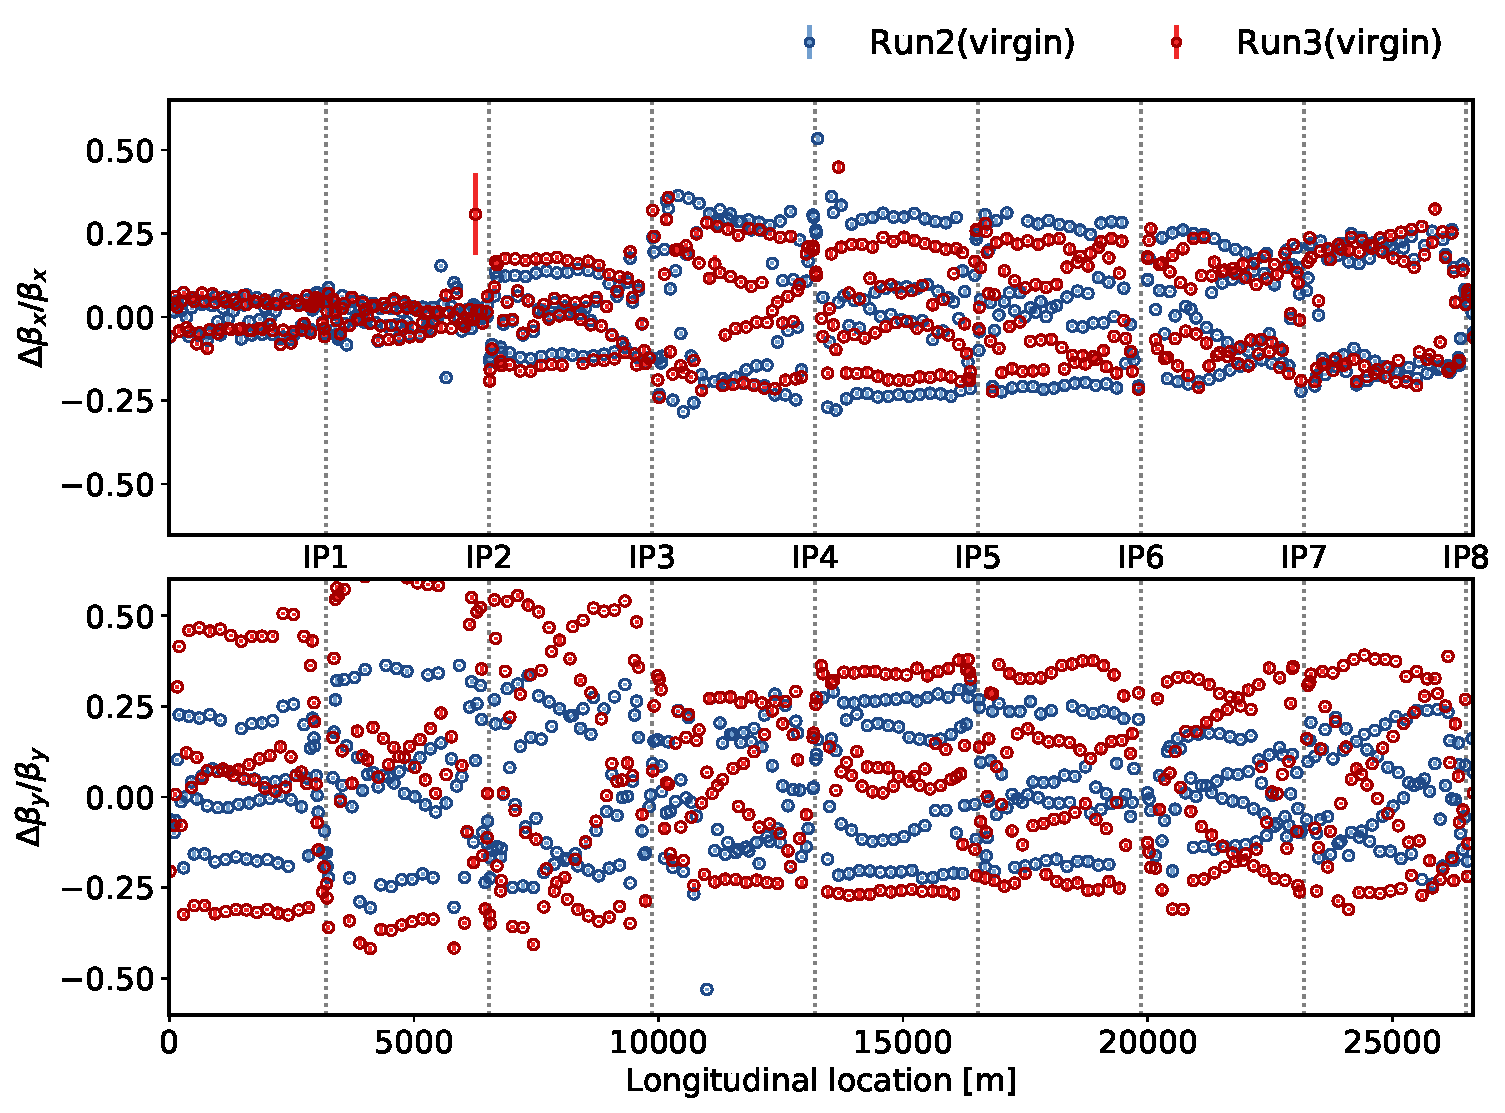
\includegraphics[width=.98\linewidth]{inj_linear/beamtest/beam2/B2_BetaBeat_2016_vs_first2021.pdf}  
  \caption{Beam~2}
\end{subfigure}
\caption{The $\beta$-beating for the first measurement in 2021 compared to the measurement in 2016 (during MD), showing a significantly increased $\beta$-beating in the vertical planes of both beams.}
\label{fig:initalVs2016}
\end{figure}
%beta_beat_before_after_pre_beam1.pdf

The first attempt was to try to understand if something had gone wrong during the pre-cycle or the fact that the machine had been around 40h at injection without any pre-cycle could have an effect. Therefore it was decided to perform a magnetic cycle to all magnets (this is called precycle) and measure optics again.
The beta-beat right after precycling and after 40h at injection is very similar, within 2-3\%, as seen in Fig.~\ref{fig:Inj_before_after_pre_cycle}.

\begin{figure}[ht]
\begin{subfigure}{.5\textwidth}
  \centering
  % include first image
  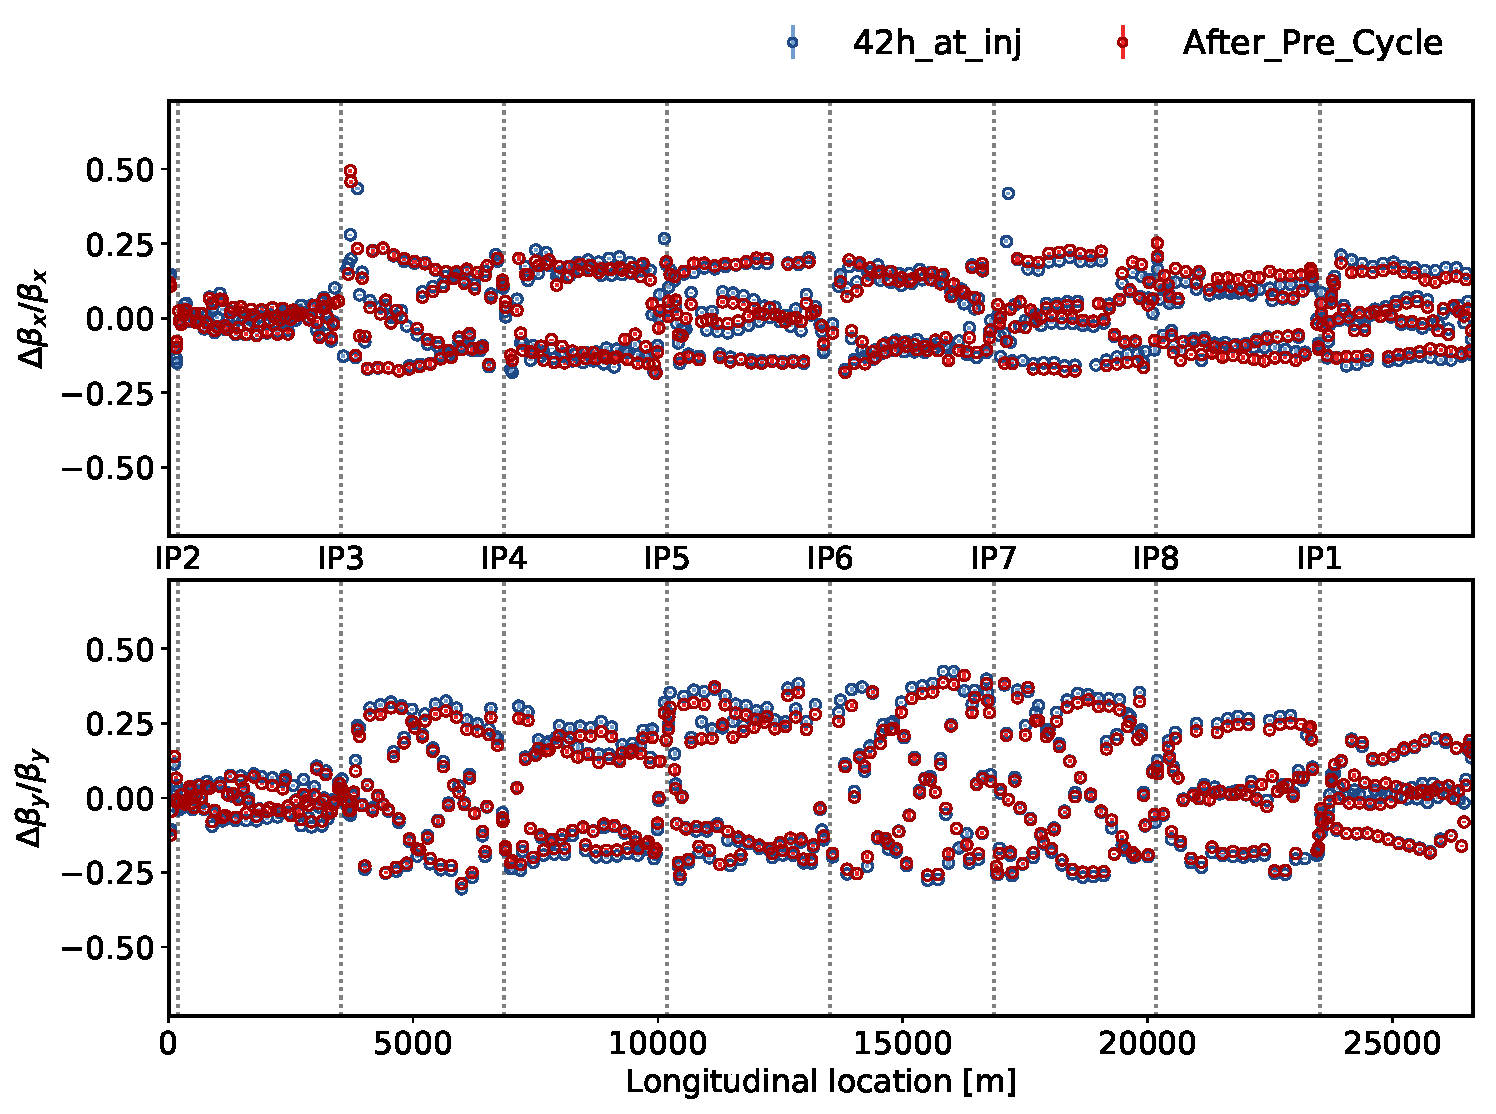
\includegraphics[width=.99\linewidth]{inj_linear/beamtest/beam1/beta_beat_before_after_pre_beam1.pdf}  
  \caption{Beam~1}
\end{subfigure}
\begin{subfigure}{.5\textwidth}
  \centering
  % include second image
  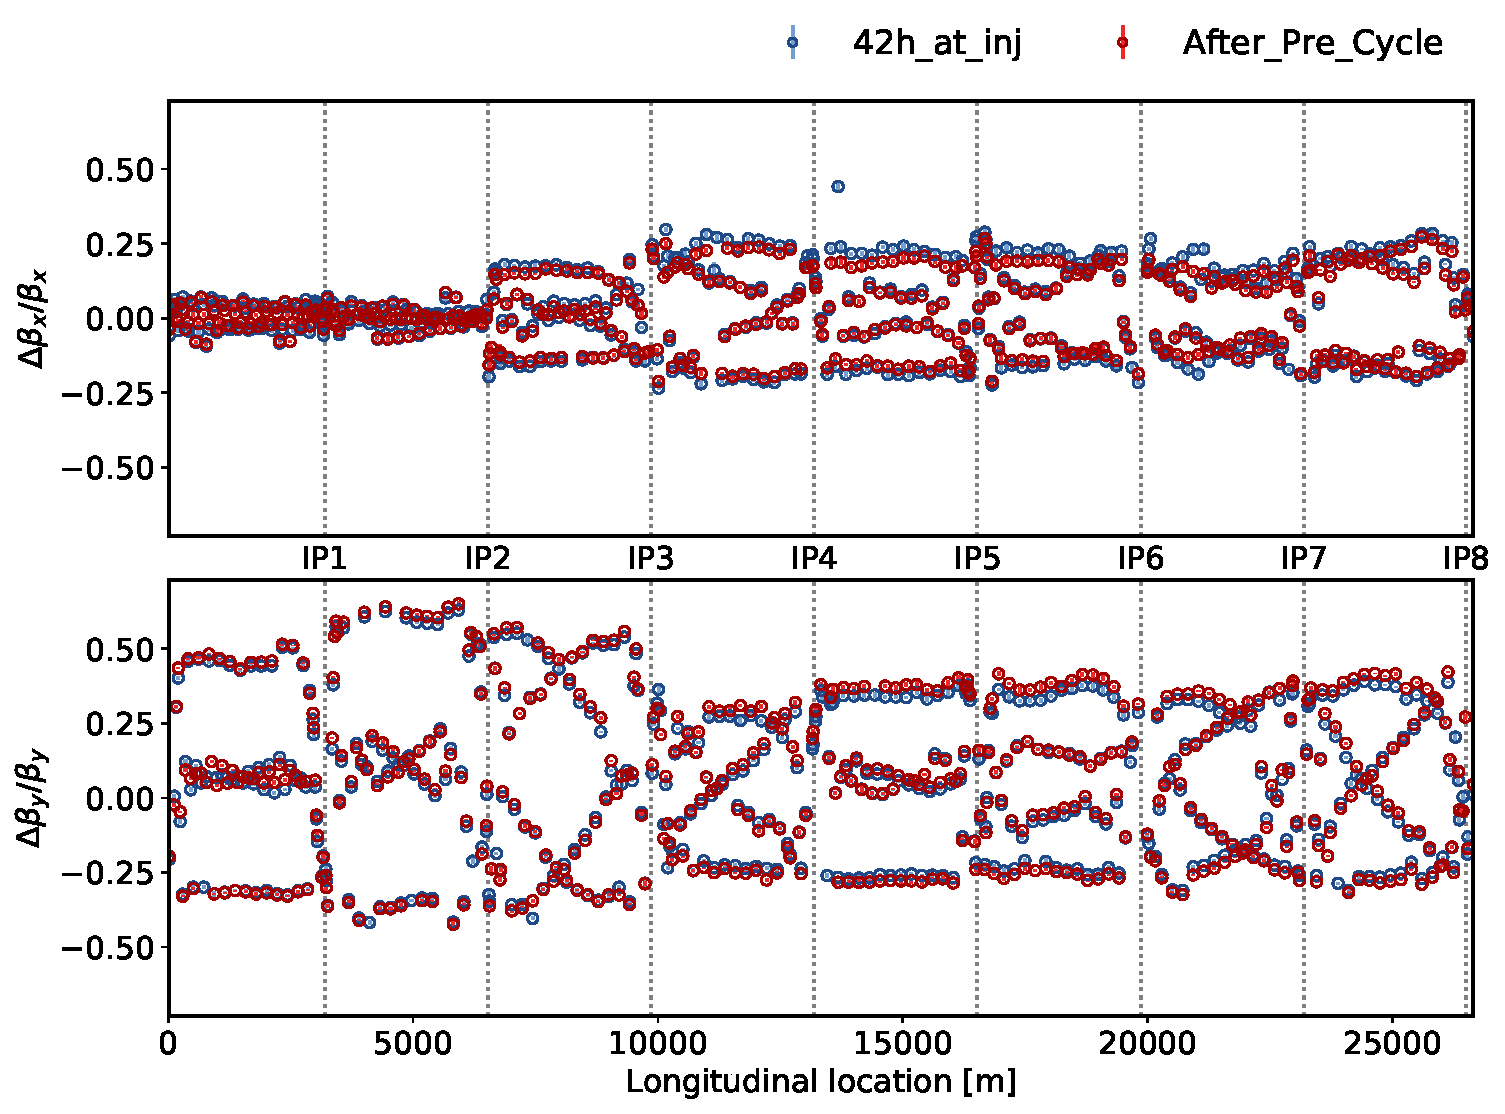
\includegraphics[width=.99\linewidth]{inj_linear/beamtest/beam2/beta_beat_before_after_pre_beam2.pdf}  
  \caption{Beam~2}
\end{subfigure}
\caption{A comparison of
$\beta$-beating right after precycling and after 42h at injection showing almost equal results within  2-3\%.}
\label{fig:Inj_before_after_pre_cycle}
\end{figure}


After ruling out that the source of the large $\beta$-beating was the extended time spent at injection we attempted to find the location of the quadrupolar error. Using the Segment-by-Segment (SBS) technique~\cite{first,tomasCERNLargeHadron2010} it was found that there was a large phase deviation in IR3 and in particular at the seventh quadrupole right of IP3, MQTL7R3.B2. It was decided that we should try to trim on that magnet in order to reduce the $\beta$-beat. The first observation was that nothing changed at all (not even a tune change). We then observed that the tune was changing on the opposite beam. We then repeated the test for the IR3Q7 of the opposite beam and we then again observed a change in tune, again on the opposite beam. From that we could conclude that indeed the IR3Q7s were swapped. This was then traced to an old swap already detected in Run~1 as reported in~\cite{first}. This was fixed at that time but then during the LS2 it was again re-introduced. After this was corrected on the software side a new measurement was carried out and the $\beta$-beat is shown in Fig.~\ref{fig:before_after_swap}. In this plot we can see that the $\beta$-beat was significantly reduced, as expected, after the swap was corrected.  

\begin{figure}[ht]
\begin{subfigure}{.5\textwidth}
  \centering
  % include first image
  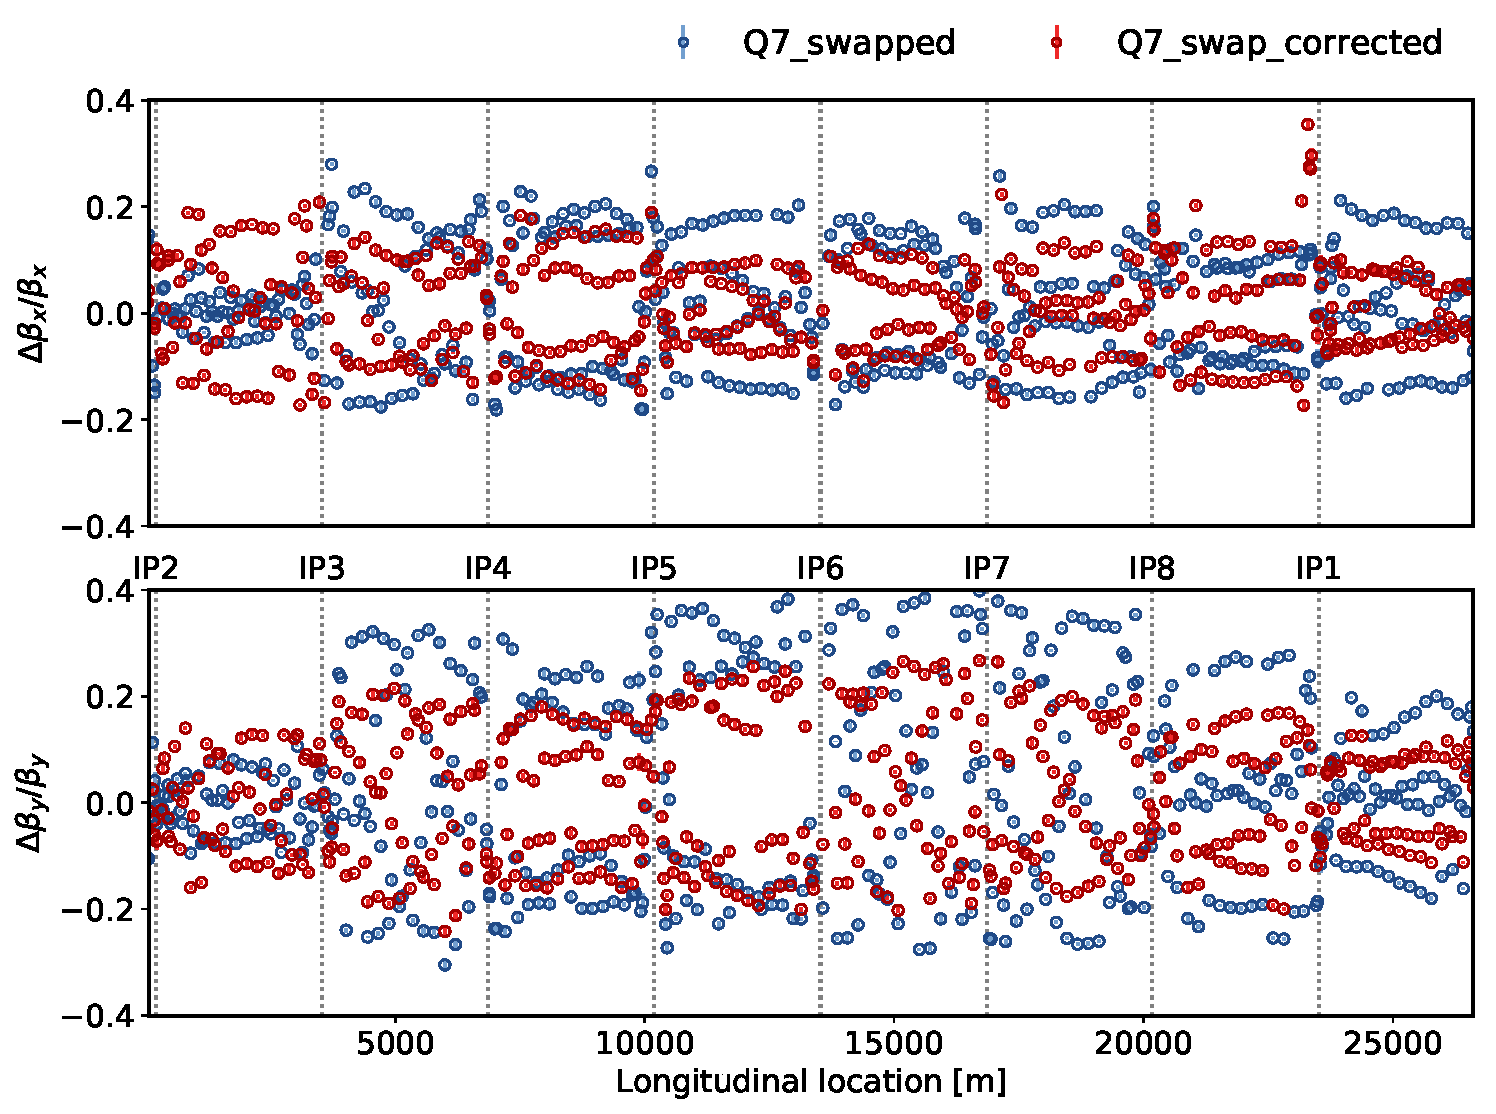
\includegraphics[width=.99\linewidth]{inj_linear/beamtest/beam1/beta_beat_before_after_swap.pdf}  
  \caption{Beam~1}
\end{subfigure}
\begin{subfigure}{.5\textwidth}
  \centering
  % include second image
  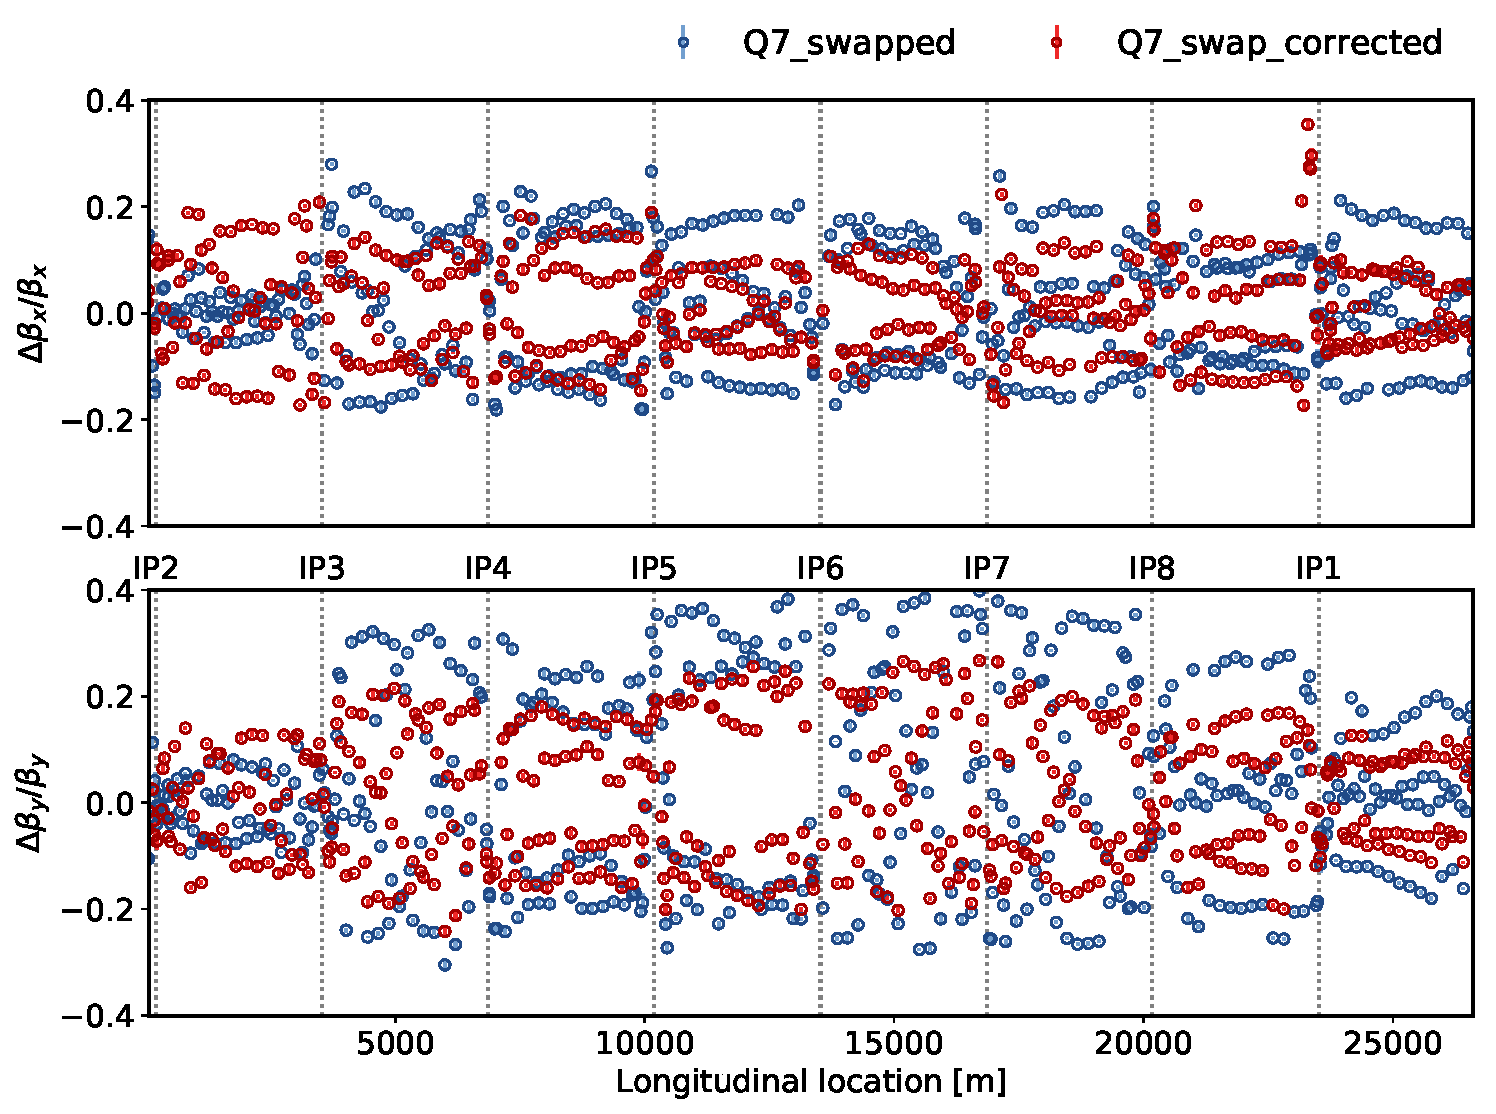
\includegraphics[width=.99\linewidth]{inj_linear/beamtest/beam1/beta_beat_before_after_swap.pdf}  
  \caption{Beam~2}
\end{subfigure}
\caption{A comparison of before and after correcting the swap of the Q7R3.}
\label{fig:before_after_swap}
\end{figure}

It is also interesting to observe if there is any sign of any degradation or any other major changes in the machine compared to Run~2. An example of a such comparison is shown in Fig.~\ref{fig:after_swap_vs_2016}. We observe that the $\beta$-beat is similar between the two measurements and the small differences can be explained from the slightly different optics and change of a few of the dipoles. 

\begin{figure}[ht]
\begin{subfigure}{.5\textwidth}
  \centering
  % include first image
  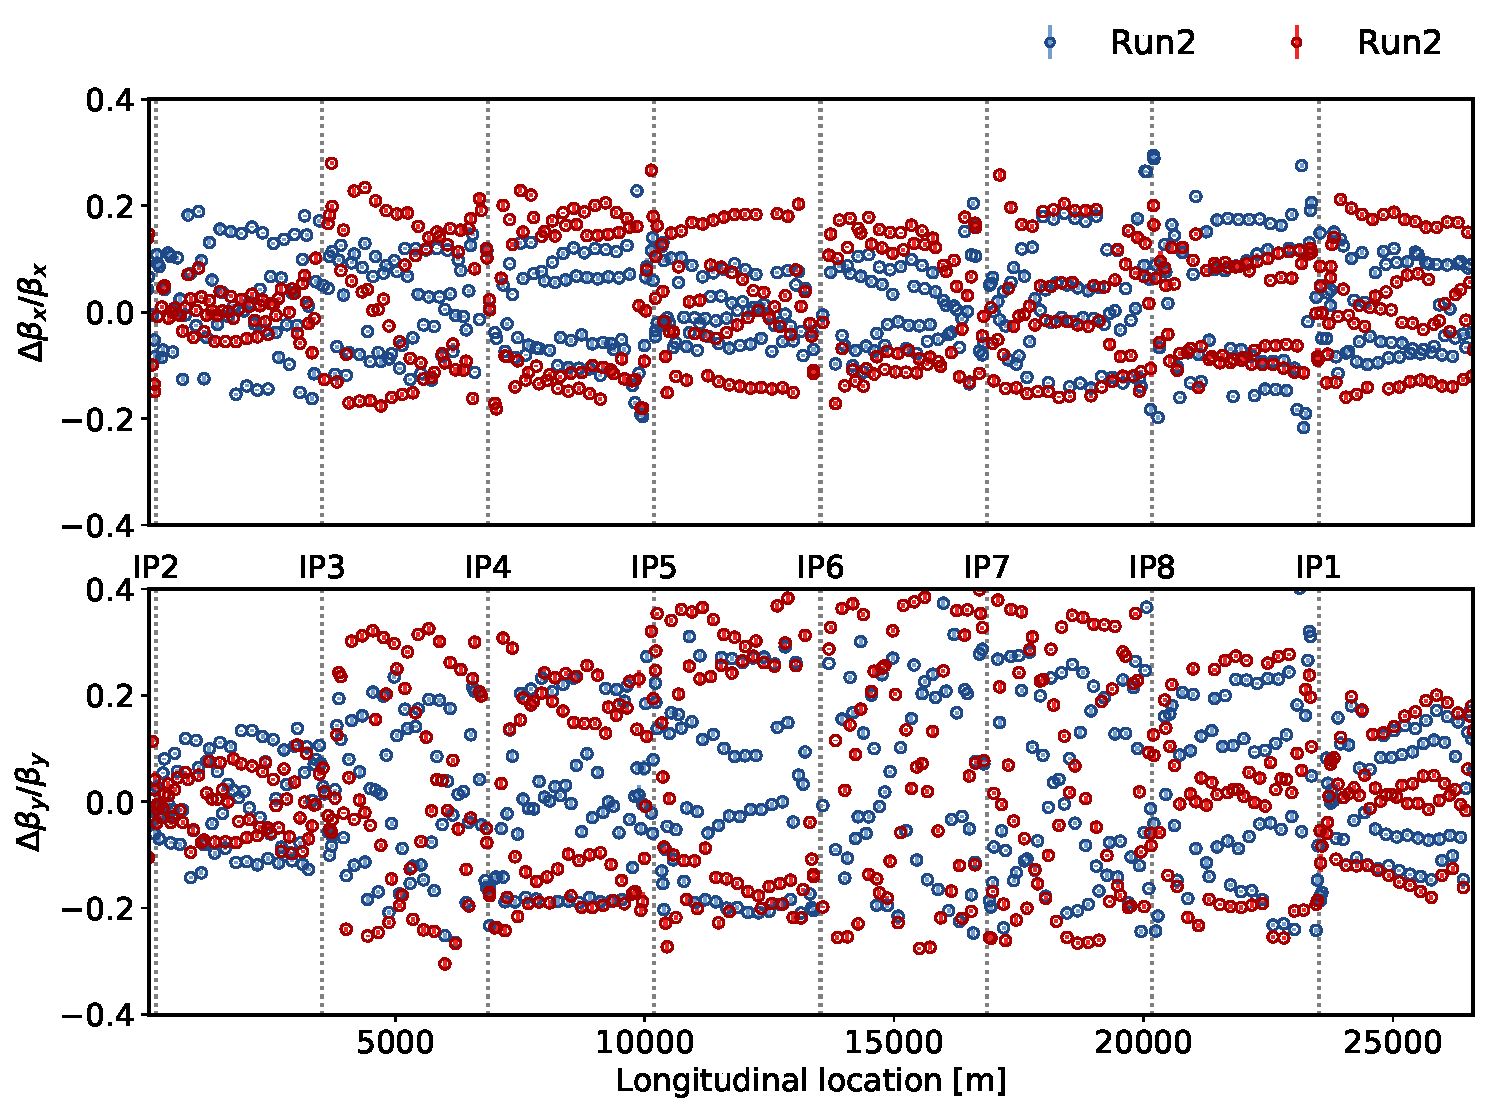
\includegraphics[width=.8\linewidth]{inj_linear/beamtest/beam1/beta_beat_virgin_2016_2021.pdf}  
  \caption{Beam~1}
\end{subfigure}
\begin{subfigure}{.5\textwidth}
  \centering
  % include second image
  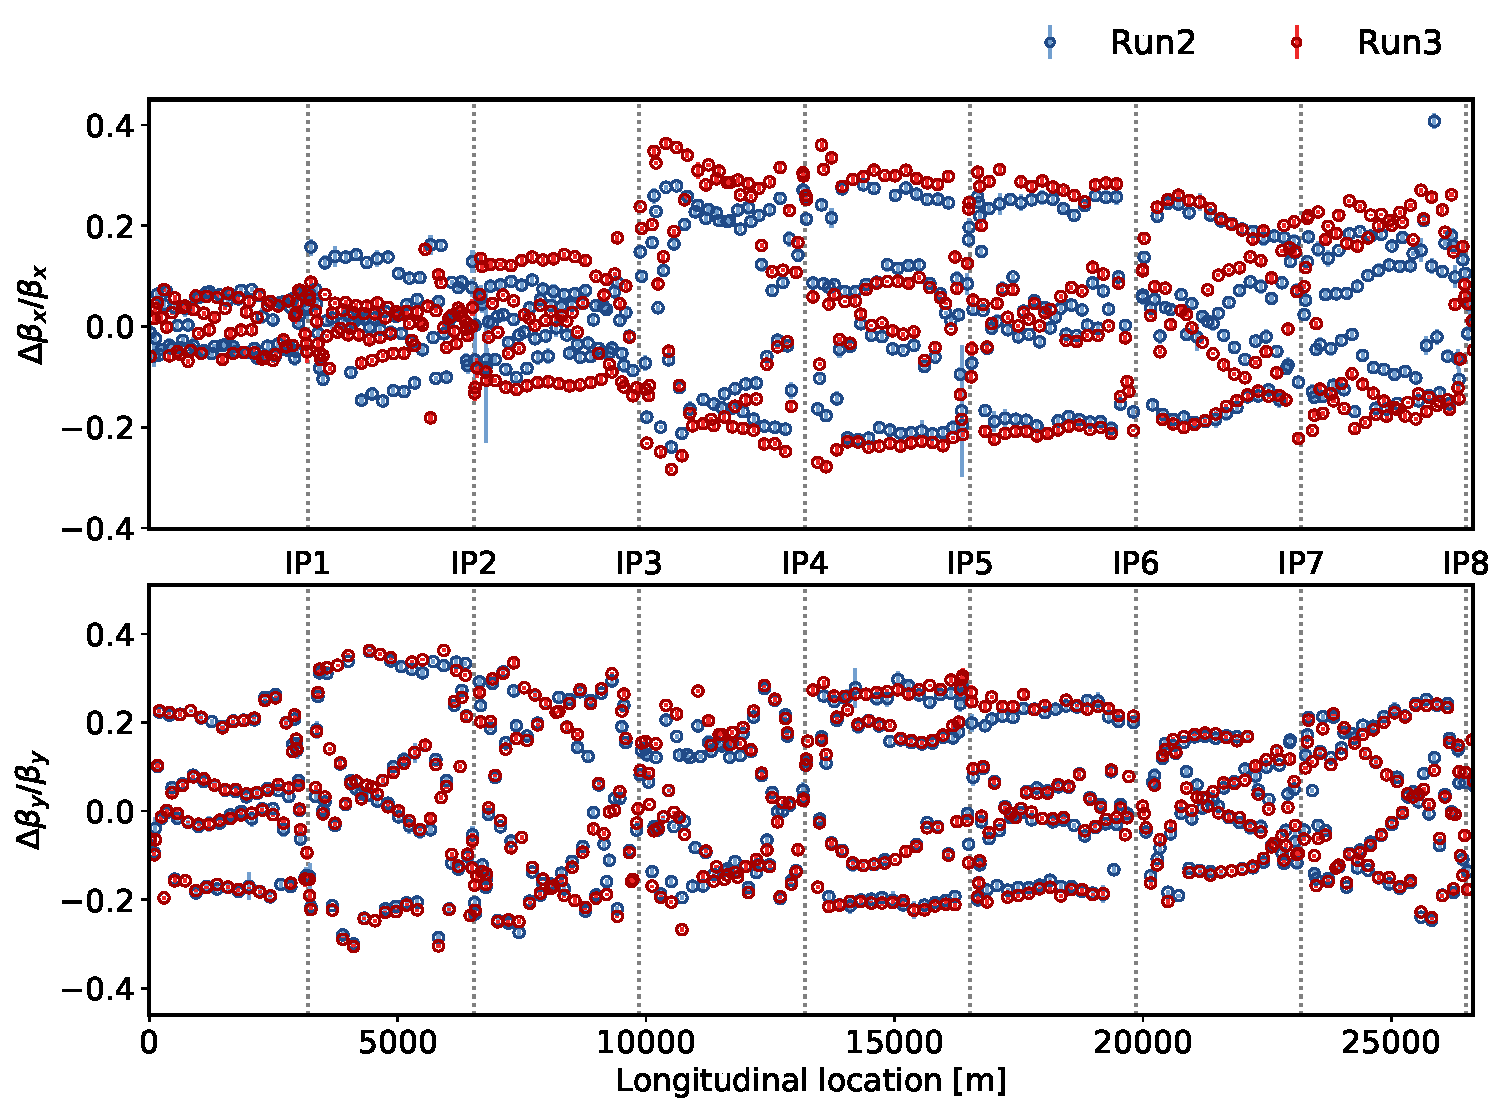
\includegraphics[width=.8\linewidth]{inj_linear/beamtest/beam2/B2_BetaBeat_afterIR3Q7fix_vs_virgin2016.pdf}  
  \caption{Beam~2}
\end{subfigure}
\caption{After fix of swap of IR3Q7 vs 2016 virgin.}
\label{fig:after_swap_vs_2016}
\end{figure}

Based on the measurement after the correction of the swapped quadrupole, a correction of the phase advance as well as the normalized dispersion was calculated. The impact on the $\beta$-beat is shown in Fig.~\ref{fig:before_after_correction_beta_beat} and the impact on the normalized dispersion is shown in Fig.~\ref{fig:before_after_correction_beta_beat}. The result is well within the required machine protection limit and similar to what has been measured as $\beta$-beat in the past. 


\begin{figure}[ht]
\begin{subfigure}{.5\textwidth}
  \centering
  % include first image
  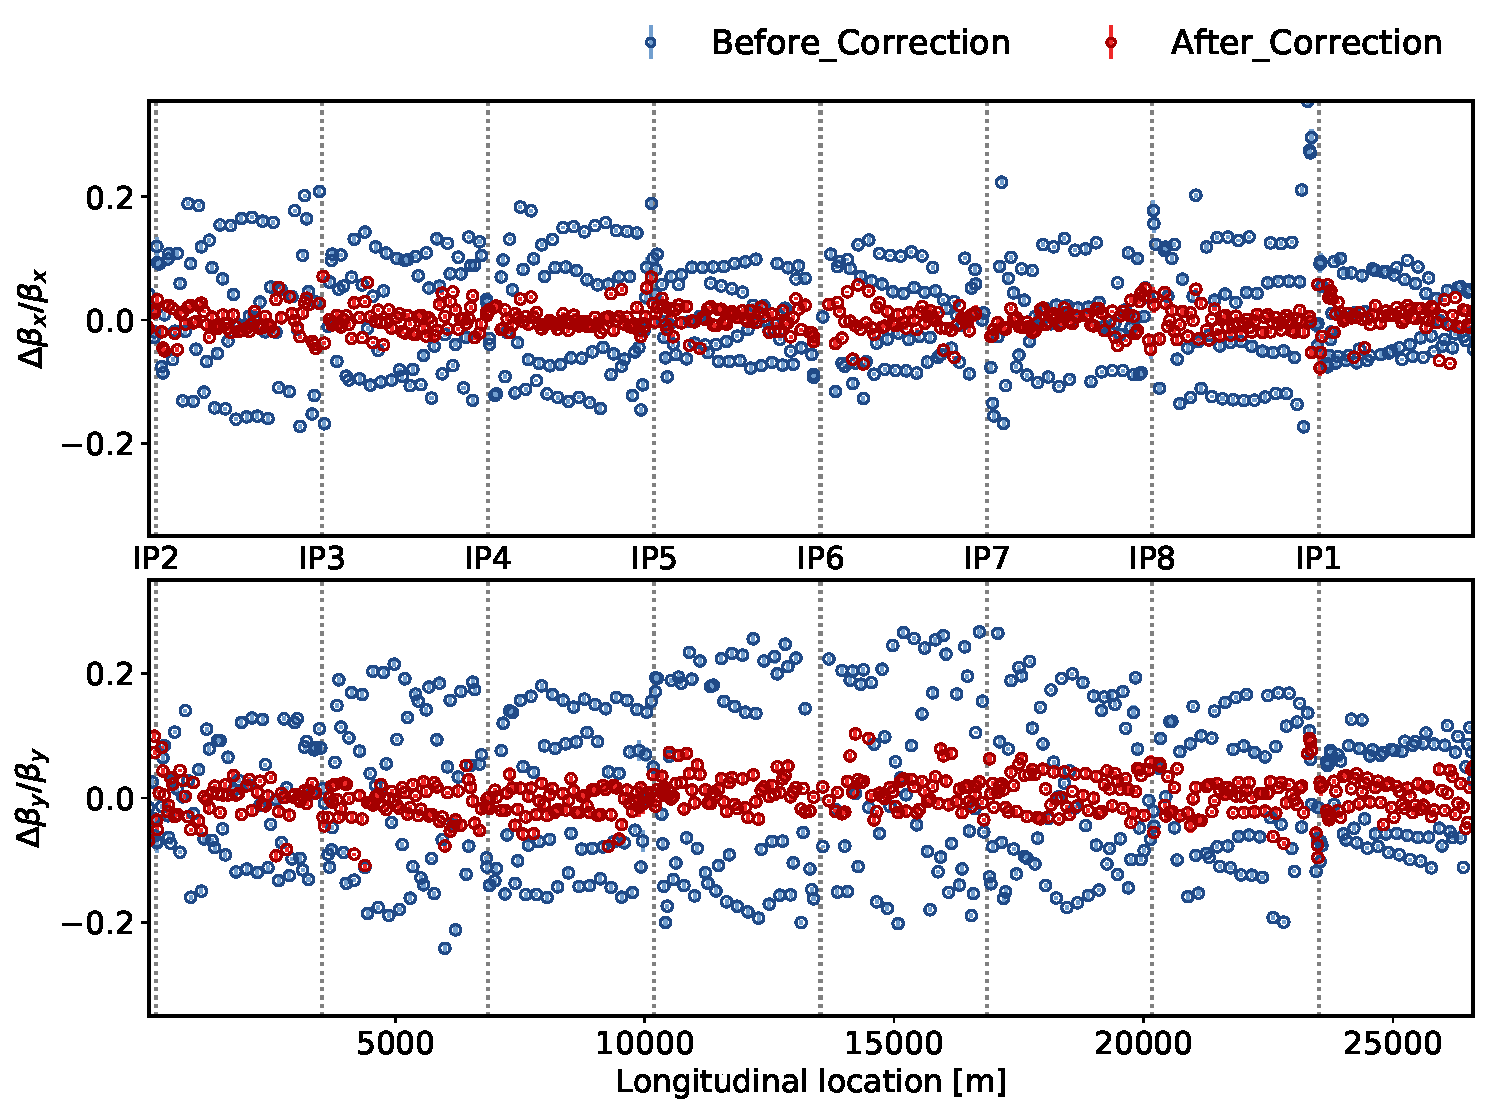
\includegraphics[width=.8\linewidth]{inj_linear/beamtest/beam1/beta_beat_before_and_after_corr.pdf}  
  \caption{Beam~1}
\end{subfigure}
\begin{subfigure}{.5\textwidth}
  \centering
  % include second image
  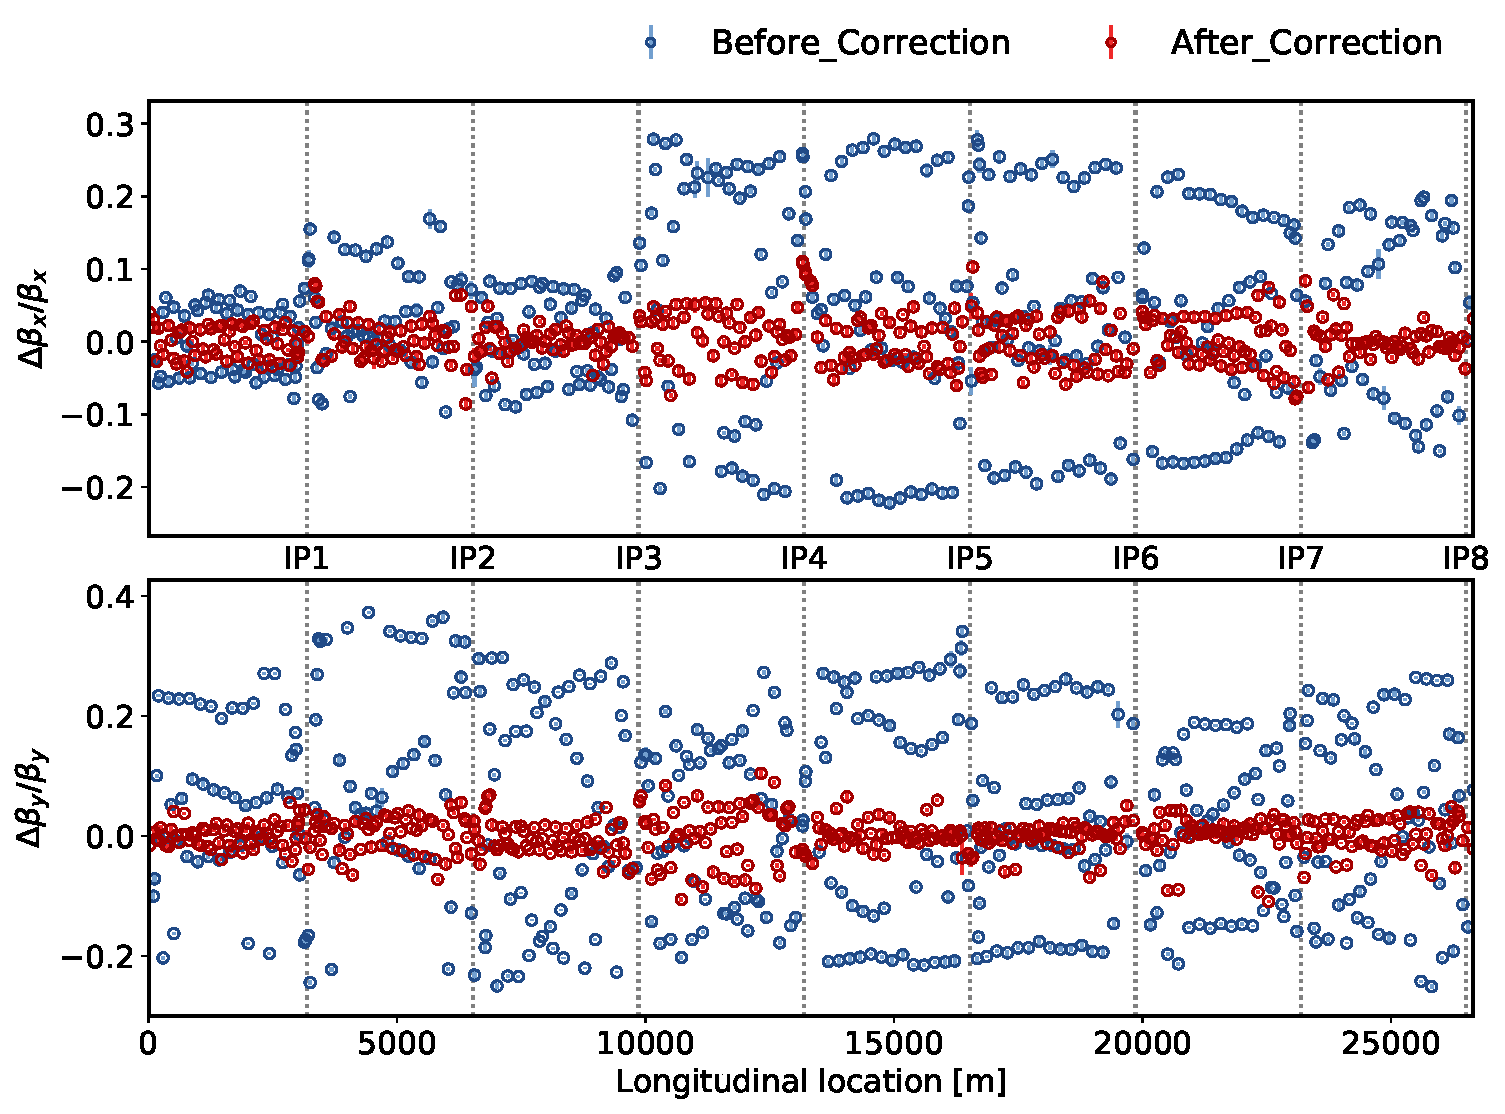
\includegraphics[width=.8\linewidth]{inj_linear/beamtest/beam2/beta_beat_before_after_correction.pdf}  
  \caption{Beam~2}
\end{subfigure}
\caption{Beta-beat before and after correction.}
\label{fig:before_after_correction_beta_beat}
\end{figure}

\begin{figure}[ht]
\begin{subfigure}{.5\textwidth}
  \centering
  % include first image
  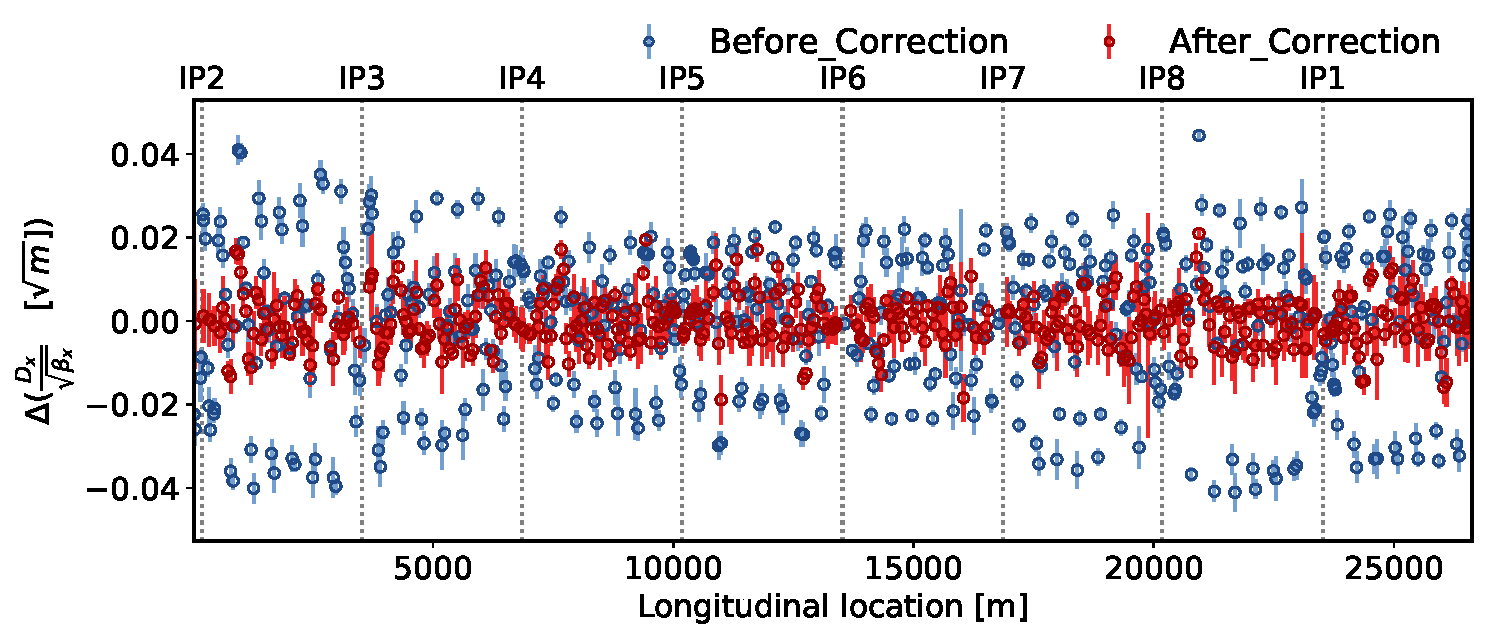
\includegraphics[width=.8\linewidth]{inj_linear/beamtest/beam1/Normalized_disp_before_vs_after_corection.pdf}  
  \caption{Beam~1}
\end{subfigure}
\begin{subfigure}{.5\textwidth}
  \centering
  % include second image
  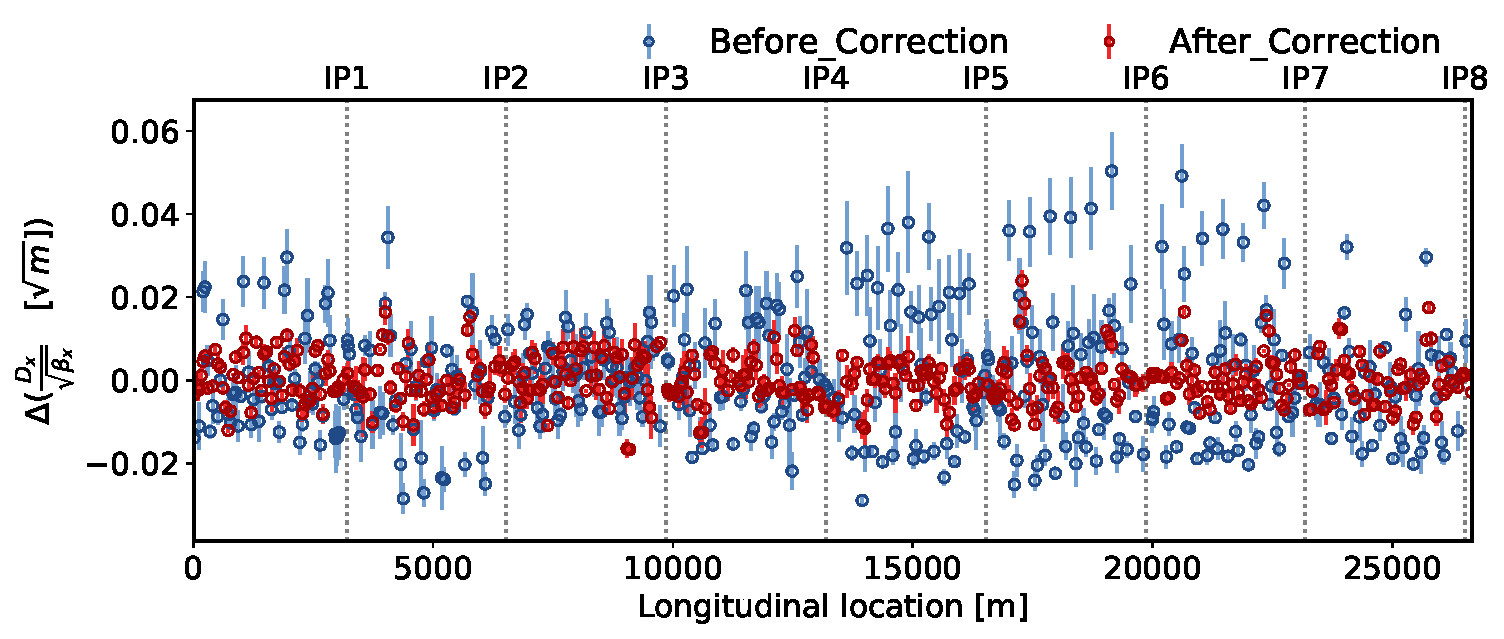
\includegraphics[width=.8\linewidth]{inj_linear/beamtest/beam2/ndisp_before_after_correction.pdf}  
  \caption{Beam~2}
\end{subfigure}
\caption{Normalized dispersion before and after correction.}
\label{fig:before_after_correction_beta_beat}
\end{figure}




\subsection{MCS powering}
\section{MCS feed-down}

It has been observed that changing the strength of the MCS ($b_3$ spool pieces) has an impact on the transverse coupling in the LHC. The main hypothesis is that this is coming from a vertical misalignment of the MCS. In order to validate if the effect had remained constraint after the Long Shutdowns a new measurement was carried out during the beam-test. The result for Beam~1 is show in in Fig.~\ref{}

\begin{figure}[ht]
\begin{subfigure}{.5\textwidth}
  \centering
  % include first image
  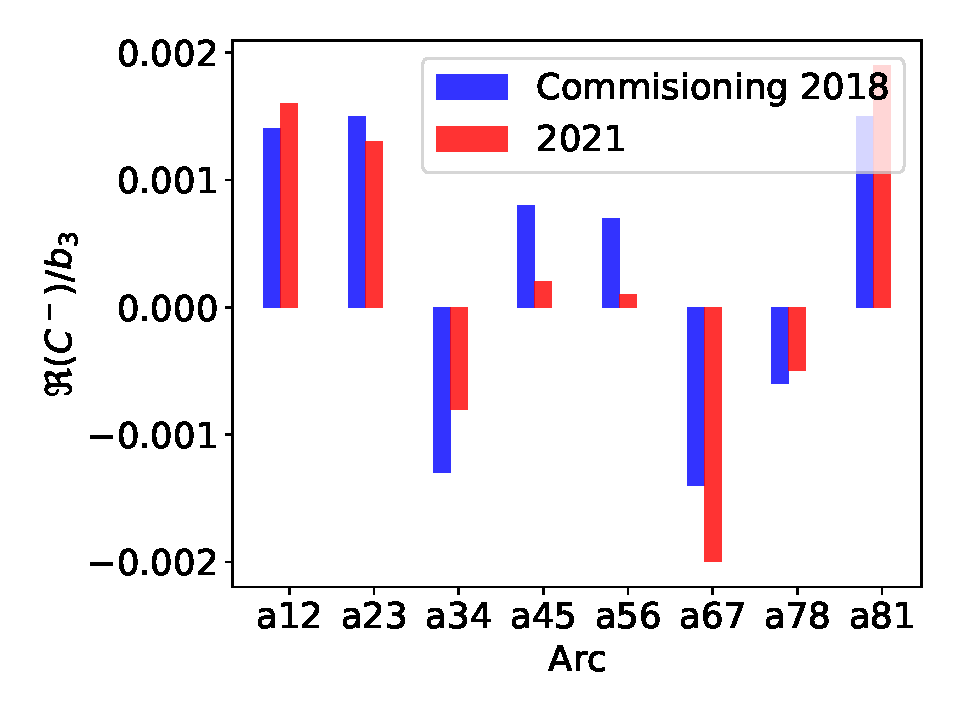
\includegraphics[width=.8\linewidth]{inj_linear/beamtest/MCS/b_1change_re_per_b3.pdf}  
  \caption{Real part of the $C^-$.}
\end{subfigure}
\begin{subfigure}{.5\textwidth}
  \centering
  % include second image
  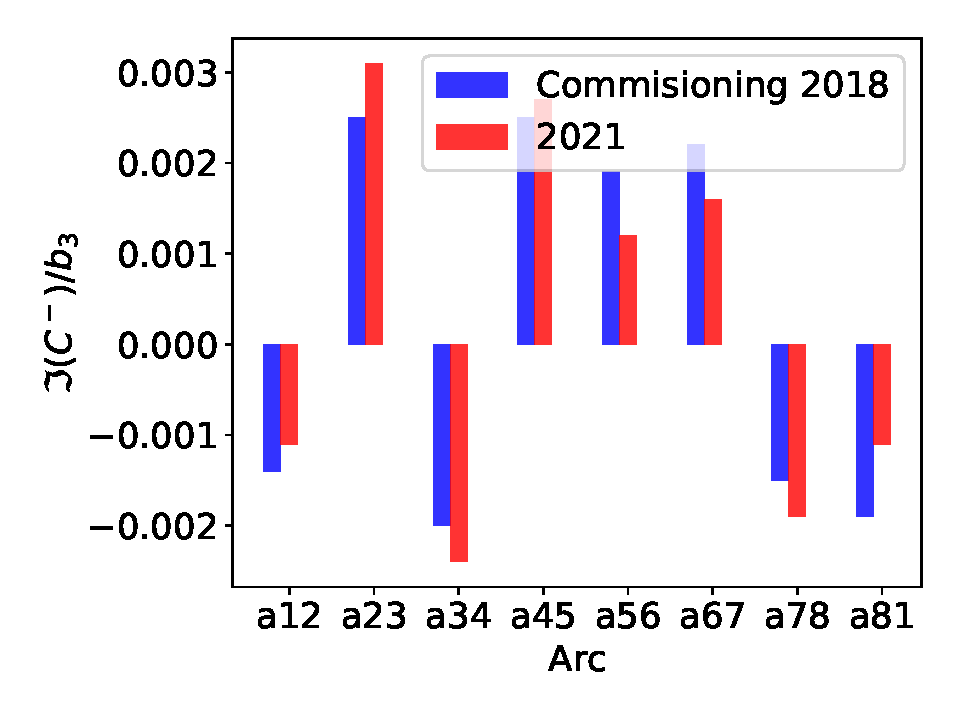
\includegraphics[width=.8\linewidth]{inj_linear/beamtest/MCS/b_1change_im_per_b3.pdf}  
  \caption{Imaginary part of the $C^-$.}
\end{subfigure}
\caption{The impact on the $C^-$ from changing the MCS corrector ($b_3$-spool pieces) for Beam~1. }
\label{fig:beam1_mcs}
\end{figure}

\begin{figure}[ht]
\begin{subfigure}{.5\textwidth}
  \centering
  % include first image
  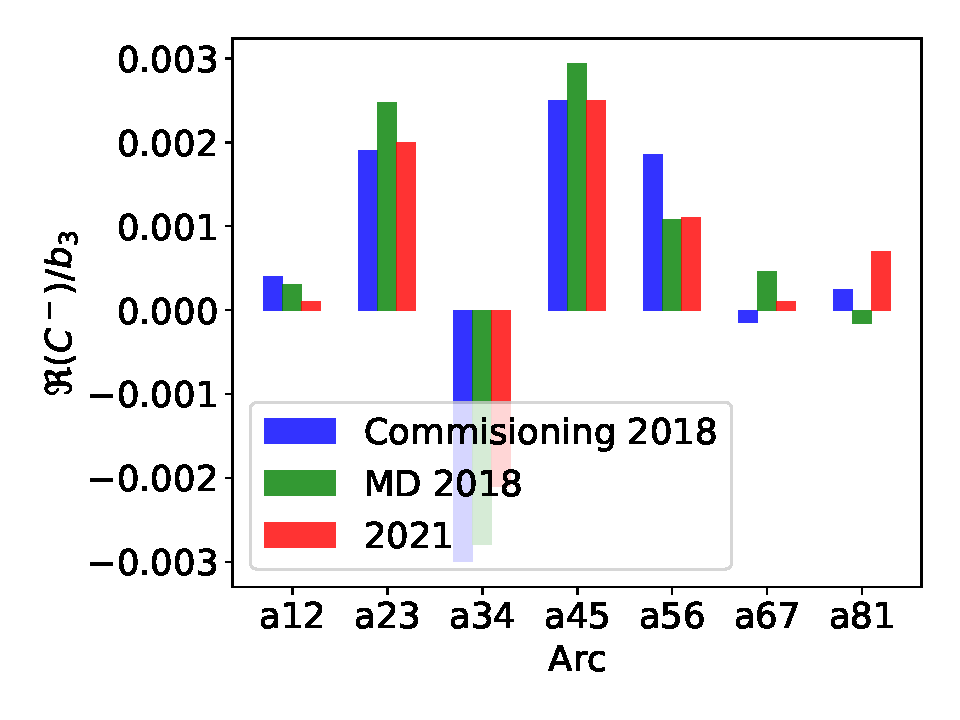
\includegraphics[width=.8\linewidth]{inj_linear/beamtest/MCS/b2_change_re_per_b3.pdf}  
  \caption{Real part of the $C^-$.}
\end{subfigure}
\begin{subfigure}{.5\textwidth}
  \centering
  % include second image
  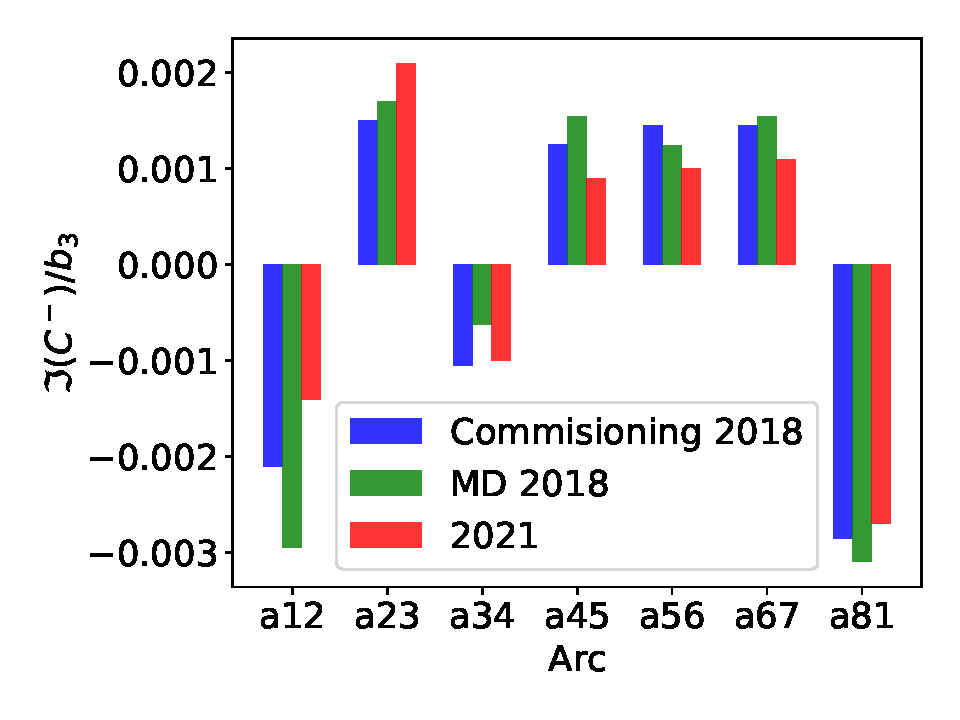
\includegraphics[width=.8\linewidth]{inj_linear/beamtest/MCS/b_2change_im_per_b3.pdf}  
  \caption{Imaginary part of the $C^-$.}
\end{subfigure}
\caption{The impact on the $C^-$ from changing the MCS corrector ($b_3$-spool pieces) for Beam~1.}
\label{fig:beam2_mcs}
\end{figure}

\subsection{Non Linear}
\section{After local corrections}
After the local corrections but before the global corrections there was a stop of YYY for the installation of the velo for LHCb. When we again measured we observed that the $\beta$-beat was significantly different to what was compared straight after the local corrections. This is shown in f

\section{Ramp}
In the beginning of Run~2 the global corrections used at injections were trimmed out linearly from 450~GeV to YYY. This was changed in 2018 because it was observed that the correction was not beneficial in the later stage. The correction was then trimmed out YYYY. This approach was also followed in the 2022 commissioning. In YYY we measured the $\beta$-beat along the ramp using 3 bunches. The use of the 3 bunches was possible due to a simulation that considered the machine protection during LS~2\cite{}. In Fig~\ref{fig:ramp_peak_rms} is shown. We notice that there is a peak close to which is a bit higher around 1900~GeV in horizontal and around 3000~GeV in vertical. 

\begin{figure}[ht]
\begin{subfigure}{.5\textwidth}
  \centering
  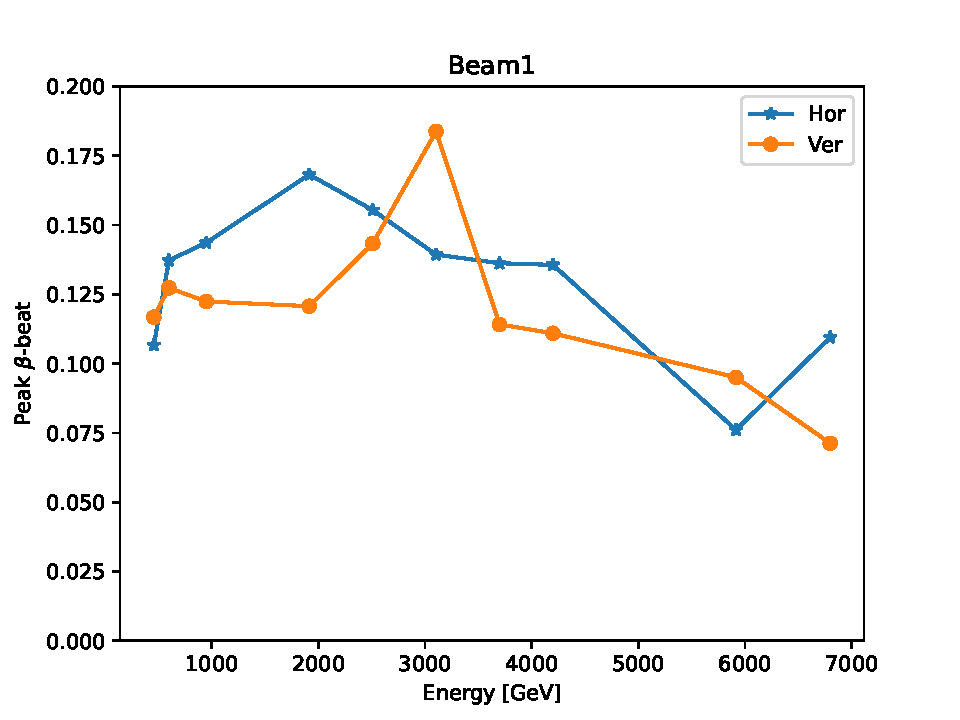
\includegraphics[width=.8\linewidth]{ramp/Beam1_peak_filter.pdf}  
  \caption{Beam~1 peak $\beta$-beat at the different energies during the ramp in 2022.}
\end{subfigure}
\begin{subfigure}{.5\textwidth}
  \centering
  % include second image
  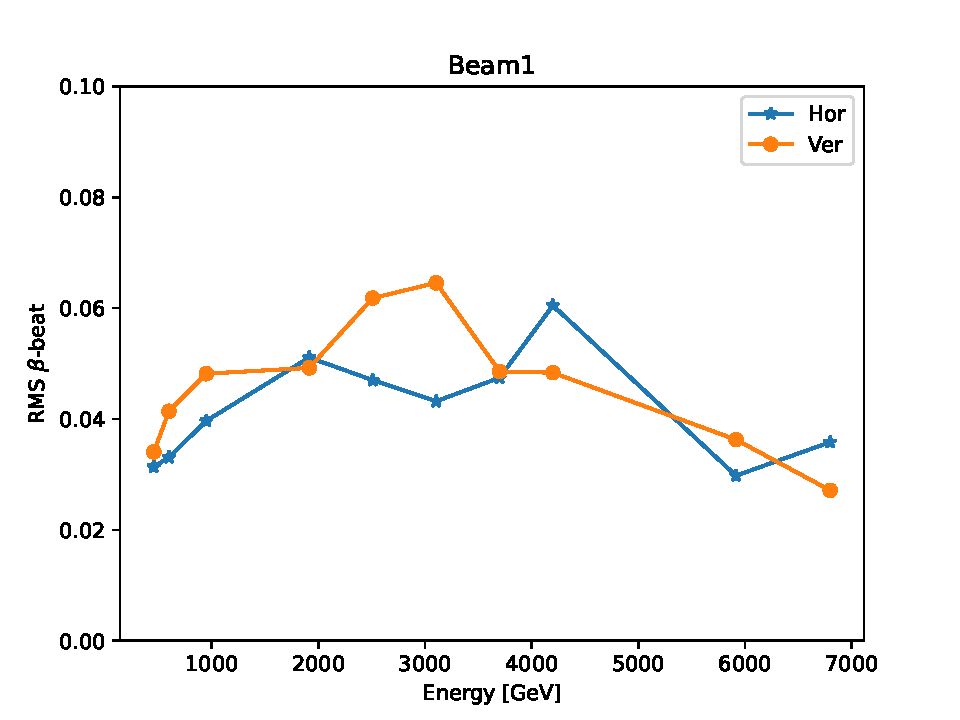
\includegraphics[width=.8\linewidth]{ramp/Beam1_rms_filter.pdf}  
  \caption{Beam~2}
\end{subfigure}
\caption{$\beta$-beat with the LRBB wire On and Off.}
\label{fig:ramp_peak_rms}
\end{figure}

In Fig.~\ref{fig:ramp_mqt} the $\beta$-beat is plotted together with the expected $\beta$-beat from the powering of the MQTs. We can observe that for the peak values they add up in phase with the measured large values. The MQTs are used to correct the tune along the cycle. A difference in how they are operated this year is that the knobs used for tune correction are only utilizing the non-ATS arcs for the corrections. This makes the strength of the magnets stronger which then in turn has a bigger impact on the $\beta$-beat. The $\beta$-beat was still considered to be within a good level and no dedicated correction is needed. However, in view of 2023 it is worth considering of applying a correction.

\begin{figure}[ht]
\begin{subfigure}{.5\textwidth}
  \centering
  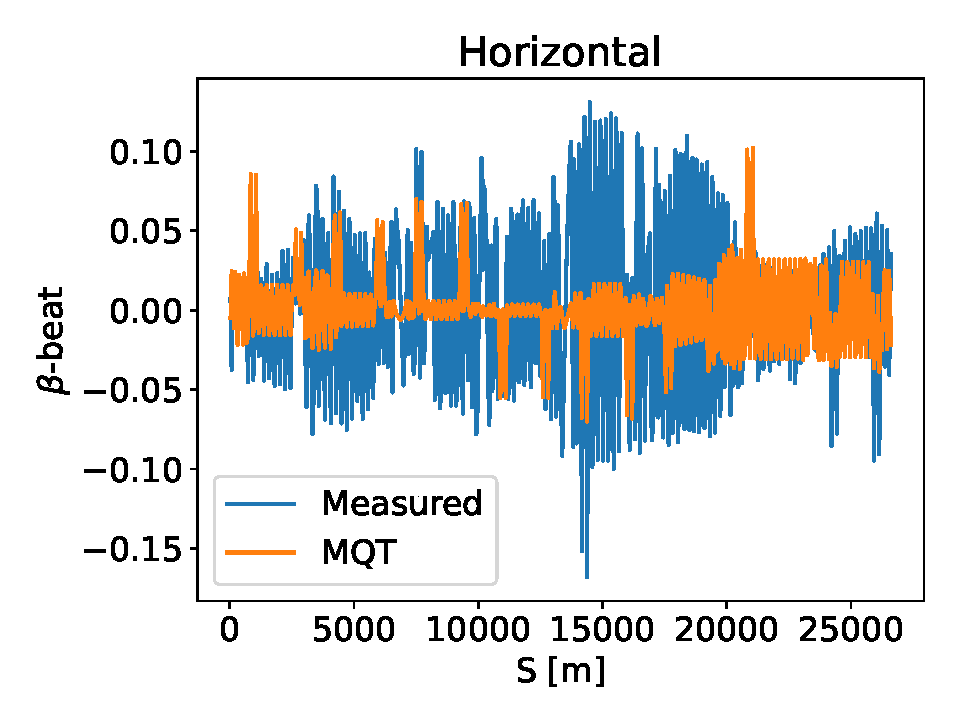
\includegraphics[width=.8\linewidth]{ramp/mqt_in_ramp_1900GeV_horizontal.pdf}  
  \caption{Beam~1 peak $\beta$-beat at the different energies during the ramp in 2022.}
\end{subfigure}
\begin{subfigure}{.5\textwidth}
  \centering
  % include second image
  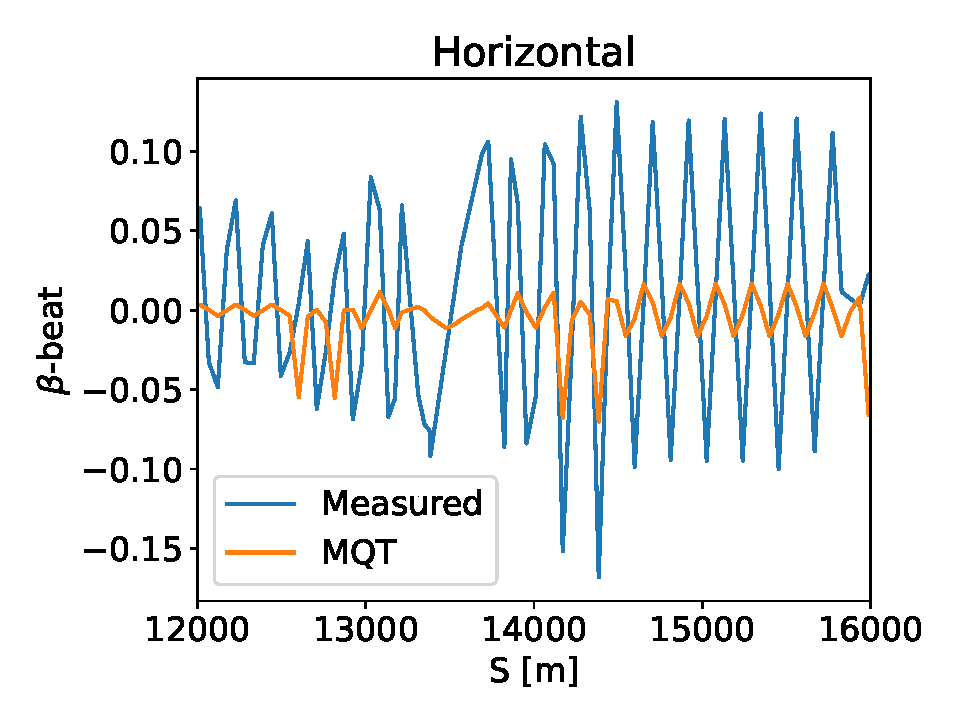
\includegraphics[width=.8\linewidth]{ramp/mqt_in_ramp_1900GeV_horizontal_zoom.pdf}  
  \caption{Beam~2}
\end{subfigure}
\caption{$\beta$-beat with the LRBB wire On and Off.}
\label{fig:ramp_mqt}
\end{figure}

\section{Local}

In order to determine the Interaction Region local corrections the optics were squeezed down to $\beta^*$ = 30~cm without any optics corrections. This is the smallest $\beta^*$ ever reached in the LHC without triplet corrections. The measurement revealed a peak $\beta$-beating of around 150\% which is also the highest ever measured in the LHC. The usual procedure to compute local IR corrections was followed. It consists of taking turn-by-turn data with the AC-dipole~\cite{record} and performing K-modulation for the most inner quadrupole (Q1) left and right of IP1 and IP5~\cite{felixkmod}. 
The local corrections calculated in Run~2 were all based on the SbS technique~\cite{tomasCERNLargeHadron2010, jaime_rdt}. In Run~3 two additional methods based on Action-Phase-Jump (APJ)~\cite{cardona17, cardona20,Garcia_Morales:IPAC21-MOPAB186, ipac2022_apj} and Machine Learning (ML)~\cite{IPAC2020Fol , epj_efol, efol_mlcorr_this_conference} were used. The SbS and APJ techniques are using both the AC-dipole turn-by-turn data and the results from the K-modulation while the ML currently only uses the Turn-by-Turn (TbT) data. The three different methods performed well but the ML was less local in the correction and therefore the choice was then between the SbS and APJ. Even though the corrections are different in strength, see Tab.~\ref{tab:localcorr:full}, they had almost identical impact on both the phase and the $\beta$-functions, as seen in Fig.~\ref{fig:local_ip15}. We can also observe that the corrections calculated in Run~2 were not fully compatible with what was measured in Run~3~\footnote{The compared corrections are from the proton-proton run. A small correction was also applied for the Ion Run in 2018~\cite{tobias_evian19}}. The difference of the local phase beating between Run 2 and Run 3 is smaller than what was observed between Run~1 and Run~2~\cite{evian_2015_langer}.
\begin{table}
    \centering
    \caption{\label{tab:localcorr:full} Local correction strengths for end of proton Run~2 compared values calculated using APJ and SbS in Run~3. The polarity indicates the sign of the $K$-value of the magnet.} 
    \begin{tabular}{l|lSSS|c|} \toprule
          & \textbf{Circuit}%
          & \multicolumn{3}{c|}{$\Delta k (10^{-5}\SI{}{m^{-2}})$}
          %\multicolumn{3}{c|}{$\bm{\Delta k}$ \textbf{($\bm{10^{-5}}$\textbf{m}$\bm{{}^{-2}}$)}} %
          & \textbf{Polarity}%
        \\ \cmidrule{2-6}
          &
          & \multicolumn{1}{c}{\textbf{Run 2}} &{\textbf{APJ}} &{\textbf{SbS}}
          & \textbf{LSA} \\\hline \midrule
        %ktqx2.r1 + 1.7e-6 (MAD-X values to match the errors)
        %ktqx2.l1 - 1.7e-6
 IR1 & \textbf{ ktqx1.l1}  &  1.23 &  0    &  1.23 & - \\
     & \textbf{ ktqx1.r1}  & -1.23 &  0    & -1.23 & +\\
     & \textbf{ ktqx2.l1}  &  0.65 &  1.15 &  0.41 & +  \\
     & \textbf{ ktqx2.r1}  & -1.0  & -0.87 & -0.70 & - \\
     & \textbf{ ktqx3.l1}  &  1.22 &  1.94 &  1.22 & - \\
     & \textbf{ ktqx3.r1}  & -1.22 & -2.88 & -1.22 & +\\\hline \midrule
 IR5 & \textbf{ ktqx1.l5}  &  2.0  &  0    &  2.25 &  -\\
     & \textbf{ ktqx1.r5}  & -2.0  &  0    & -2.10 & +\\
     & \textbf{ ktqx2.l5}  &  0.26 &  0.38 &  0.16 & +\\
     & \textbf{ ktqx2.r5}  &  1.48 &  0.93 &  1.35 & -\\
     & \textbf{ ktqx3.l5}  &  1.49 &  3.40 &  2.25 & -\\
     & \textbf{ ktqx3.r5}  & -1.49 & -2.46 & -2.10 & +\\\hline \midrule

    \end{tabular}
 \end{table}
 
Both the APJ and the SbS corrections were tested in the machine and the resulting $\beta$-beating was very similar between the two sets of corrections. In Fig.~\ref{fig:30cm_before_after_local} the $\beta$-beating before and after corrections is shown. The corrections used for IP1 were calculated with APJ while for IR5 they were calculated using SbS. The reason for this was that K-modulation in this configuration gave results slightly closer to the model. Local corrections at IP2 and IP8 were also implemented, based on SbS, but they have a much smaller impact on the overall $\beta$-beating due to the larger $\beta^*$ and hence smaller $\beta$-function in the triplet magnet. 

\begin{figure}
%\begin{subfigure}{.5\textwidth}
%  \centering
  % include first image
  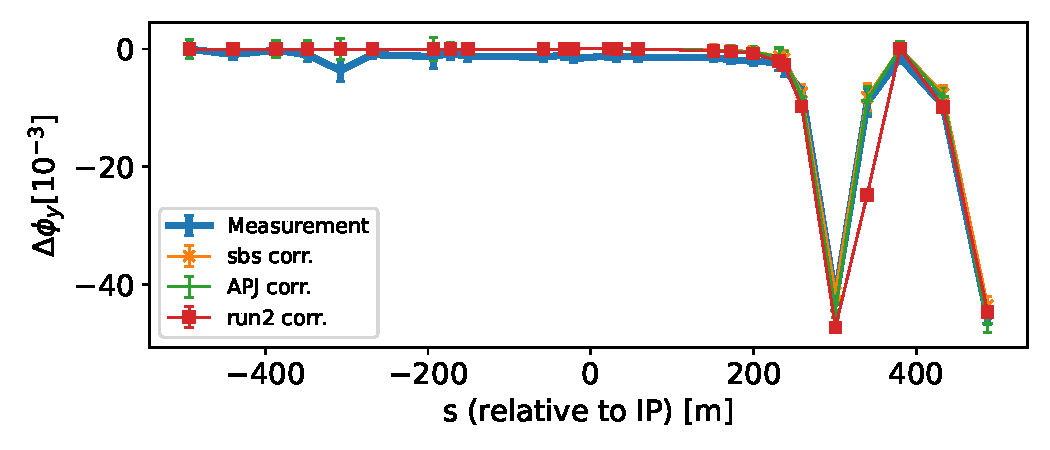
\includegraphics[width=0.5\linewidth]{local_corr/beam1_y_IP1.pdf}  
%  \caption{Beam~1 vertical}
%  \label{fig:sub_beam1_ip1}
%\end{subfigure}
%\begin{subfigure}{.5\textwidth}
%  \centering
  % include second image
  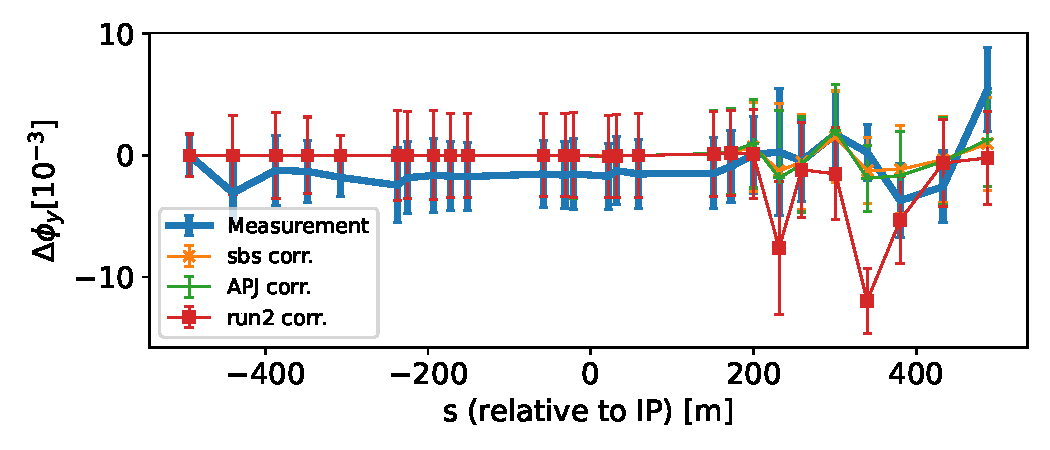
\includegraphics[width=0.5\linewidth]{local_corr/beam2_y_IP1.pdf}  
%  \caption{Beam~2 vertical}
%  \label{fig:sub_beam2_ip1}
%\end{subfigure}
%\caption{IR1 phase deviation between measurement and model run as a segment, or from a model with Run~2 corrections (with opposite sign to mimic errors).}
%\label{fig:local_ip1}
%\end{figure*}
%begin{figure*}[ht]
%\begin{subfigure}{.5\textwidth}
%  \centering
  % include first image
  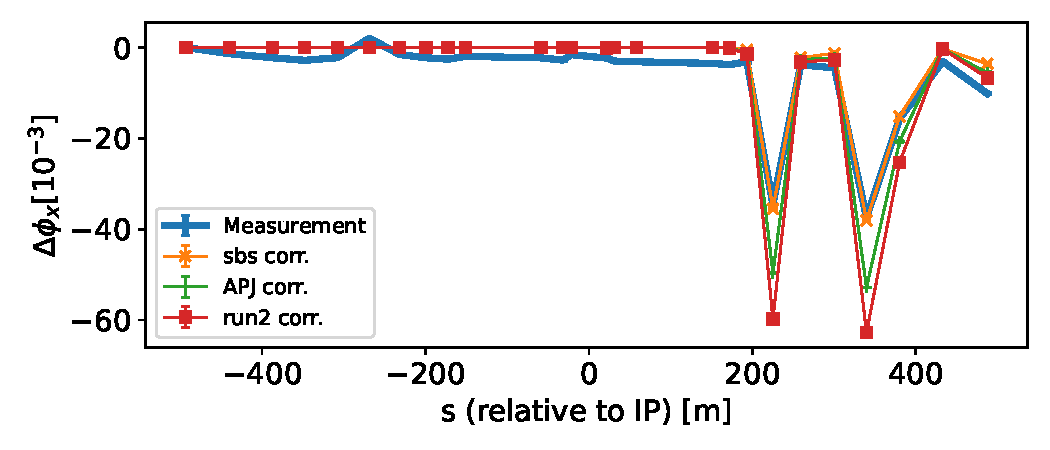
\includegraphics[width=0.5\linewidth]{local_corr/beam1_x_IP5.pdf}  
 % \caption{Beam~1 horizontal}
 % \label{fig:sub_beam1_ip5}
%\end{subfigure}
%\begin{subfigure}{.5\textwidth}
%  \centering
  % include second image
  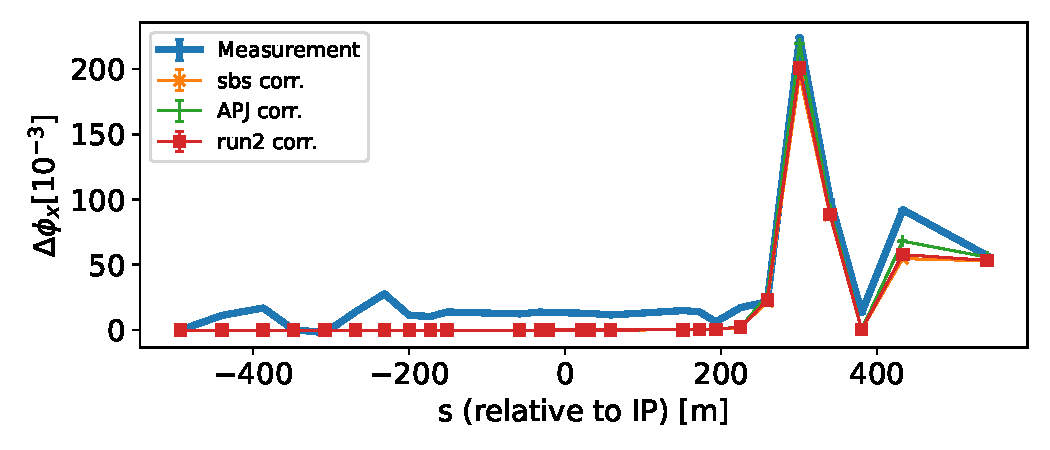
\includegraphics[width=0.5\linewidth]{local_corr/beam2_x_IP5.pdf}  
 % \caption{Beam~2 horizontal}
  %\label{fig:sub_beam2_ip5}
%\end{subfigure}
\caption{IR1 Vertical (top) and IR5 Horizontal (bottom) phase deviation between measurement and model run as a segment, or from a model with Run~2 corrections (with opposite sign to mimic errors). The left plots are for Beam 1 and right plots for Beam 2.}
\label{fig:local_ip15}
\end{figure}



\section{Wire}
The optics measurements with the LRBB were done on the 4th of August 2022. The powering was done in steps and a sign error was discovered for the compensation part for beam~2. This was quickly solved and after observing that there was no major optics change coming from the wire we did optics measurements both on- and off momentum.

An attempt to do a K-modulation was also performed but the tune signal was too noisy to draw any conclusion. The fact that the tune signal deteriorates when turning on the wire is expected because it creates an octupolar component that deteriorates the tune signal. In case it would be deemed necessary to measure the impact on the $\beta^*$ one should pre-calculate a correction of the MOF and MOD that would cancel the octupolar component of the LRBB-wire. However, from the measurement of the $\beta$-beat using the wire as well as observing the luminosity when it has been turned on in operation, it is possible to conclude that the impact must be very limited. 

\begin{figure}[ht]
\begin{subfigure}{.5\textwidth}
  \centering
  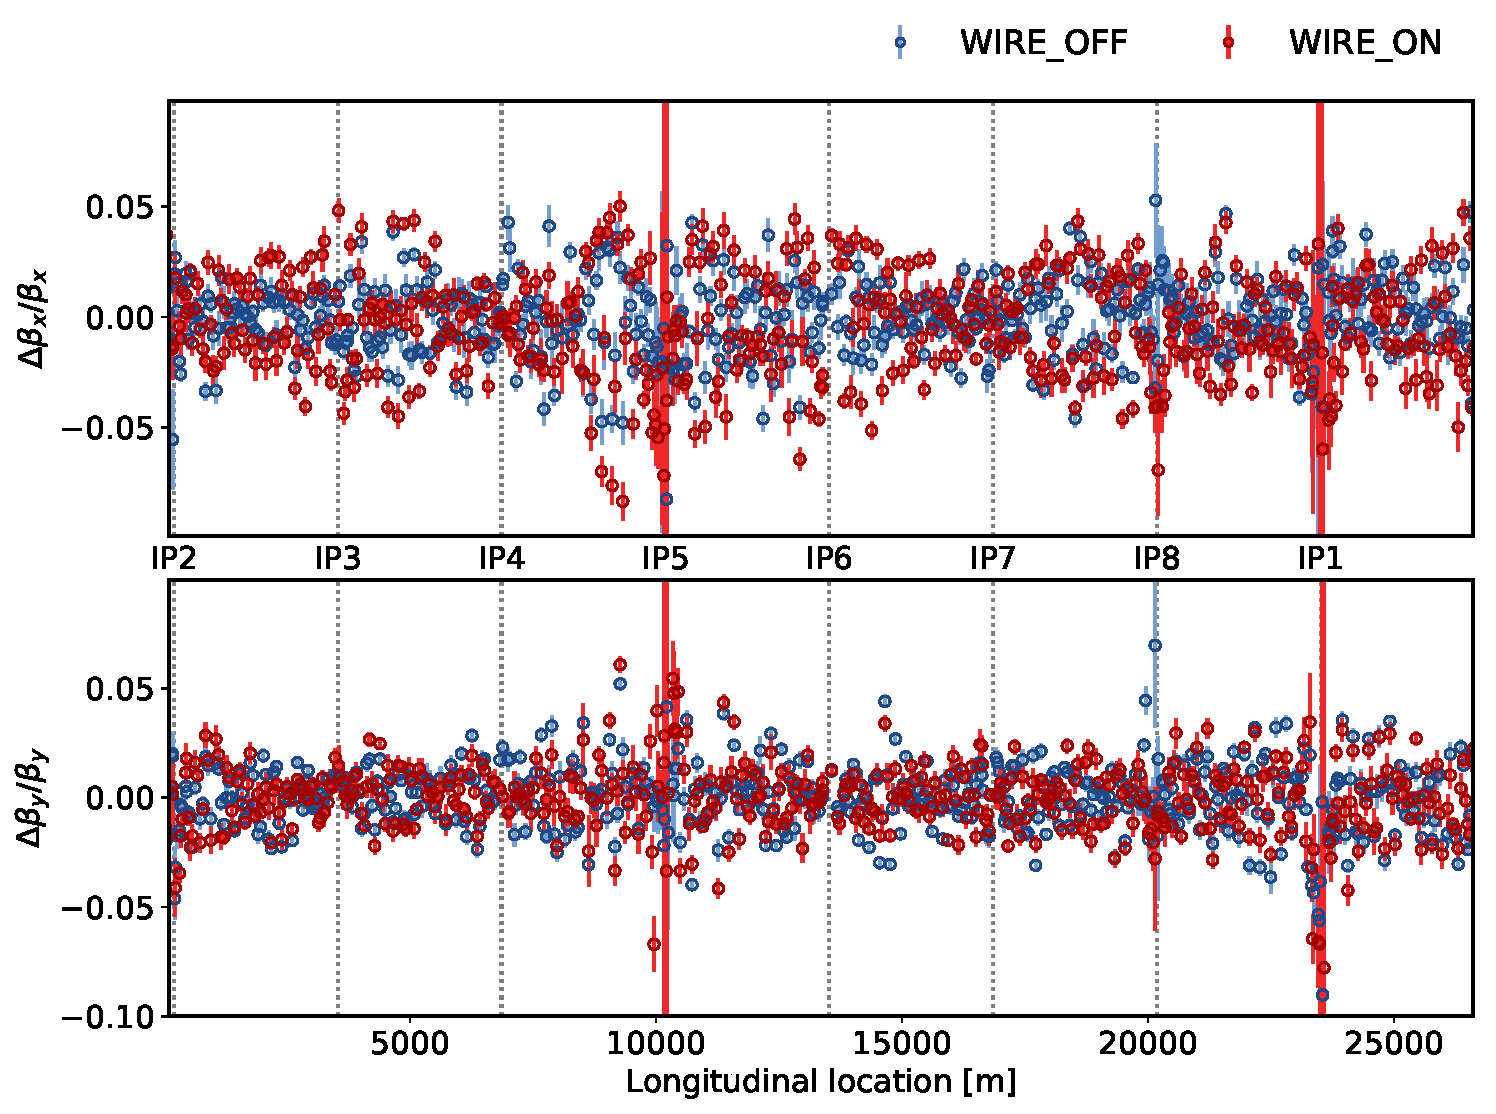
\includegraphics[width=.8\linewidth]{wire/beam1_beta_beat.pdf}  
  \caption{Beam~1}
\end{subfigure}
\begin{subfigure}{.5\textwidth}
  \centering
  % include second image
  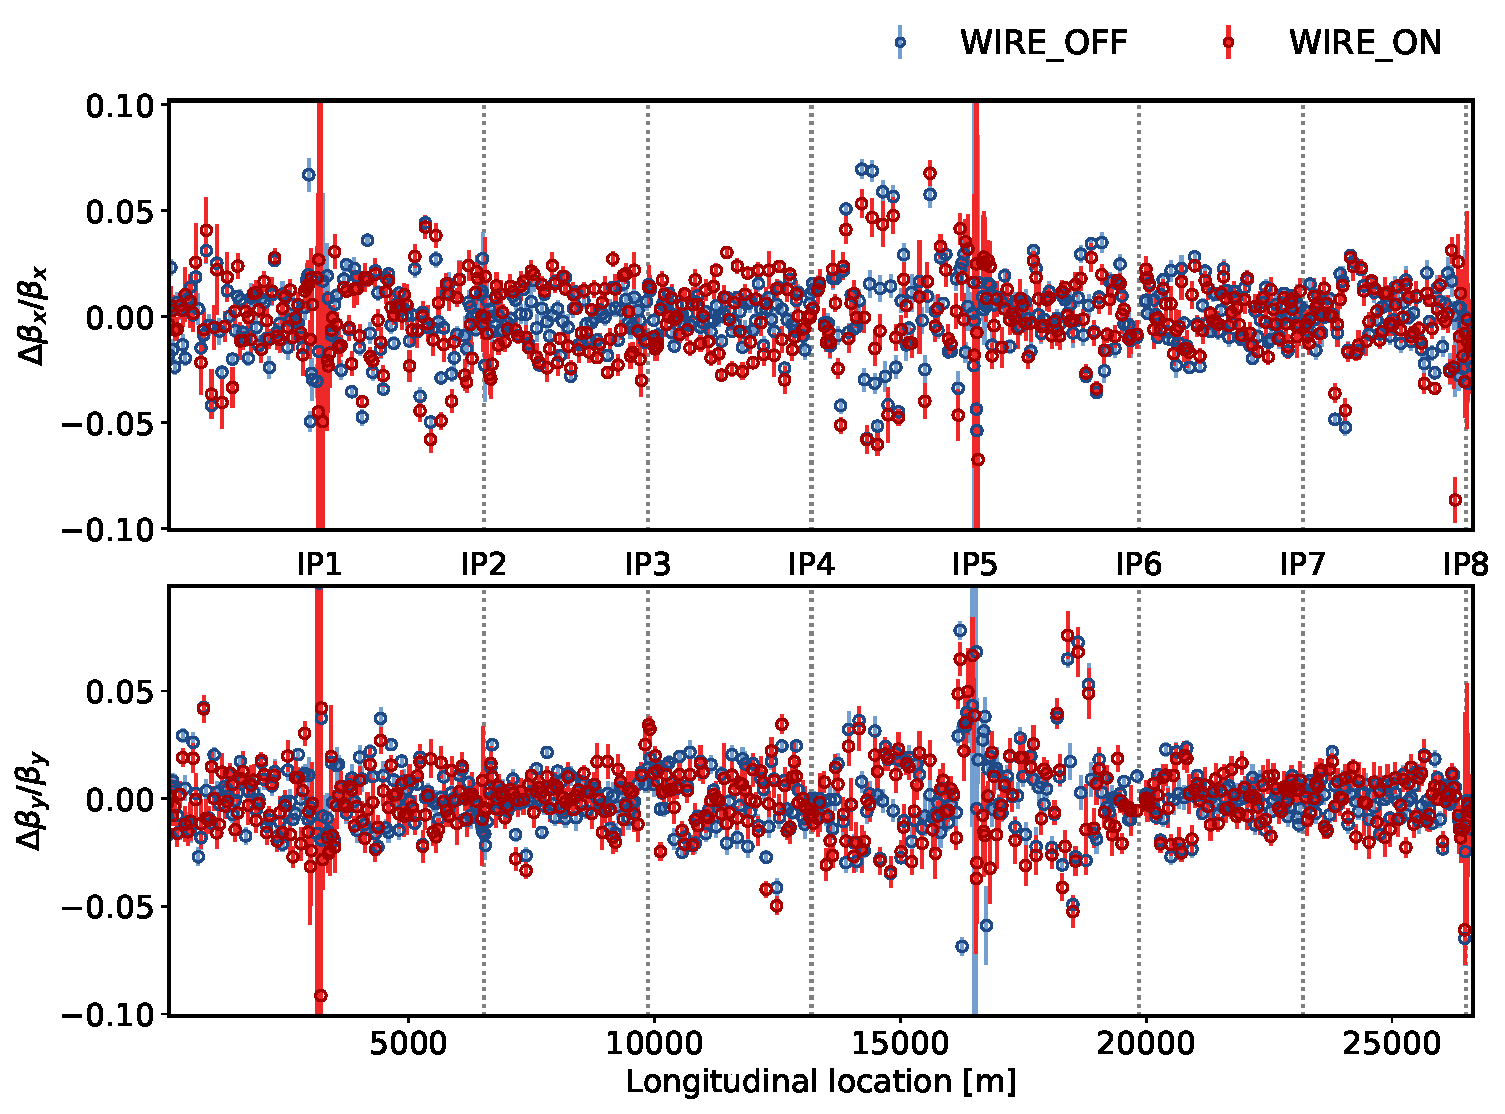
\includegraphics[width=.8\linewidth]{wire/beam2_beta_beat.pdf}  
  \caption{Beam~2}
\end{subfigure}
\caption{$\beta$-beat with the LRBB wire On and Off.}
\label{fig:before_after_pre_cycle}
\end{figure}
\section{2023}
The Run~3 optics was designed in such a way that the change between 2022 and 2023 should be small. The difference was between ~4 TeV in the ramp and down to 60~cm. The difference in this part was that while in 2022 the telescopic index was constant at 1 for this part this was first decreased to 0.5 during the ramp and then kept like that until the collisions started at 1.2~m. The other difference was in 2023 there was additional rotation of the crossing angle in IP8. 

Originally, the plan was to stay with the same injection optics in 2022 and 2023. During the yearly stop it was, however, observed that by changing the phase advance between the different sectors it would be possible to reduce the octupolar RDTs. This work and the results are described in YYY, while the injection optics measurement. 
nts and corrections from 2021 and 2022 are described in YYY1.

\section{Local coupling corrections}
The first local corrections were calculated during the beam test in 2021 based on the segment-by-segment technique. The corrections were later refined slightly for IP1 (by $10^{-4}$ for the RQXS.3L1) when the machine was squeezed down to 30cm. It is possible to balance the strength between the right and left corrector for each IP without changing the global coupling. However, the relative strength between, the two correctors has a big impact on the beam size at the IP. In order to establish the best balance between the left and right correctors two different methods were used. The first one was based on a rigid waist shift, explained in detail in YYY. The other one was based on observing the luminosity while varying the strength from the corrector on one side of the IP to the corrector on the other side. The two methods gave almost identical results for the best correction. 

\begin{table}[!htb]
    \centering
    \begin{tblr}{colspec={ccccc}}
        \hline
        \SetCell[r=2,c=1]{c} \textbf{IR}  &  \SetCell[r=2,c=1]{c} \textbf{Circuit} & \SetCell[c=3]{c} \textbf{\(K_{1\mathrm{S}}\)~[\qty{1e-4}{\per\square\meter}]}                                              \\
        \cline{3,4,5}
                                          &                                        &  \textbf{2016-2018}~\cite{CERN:Persson:LHCOpticsCorrectionsEvian2019}    &    \textbf{2022 SbS}    &    \textbf{2022 RWS}  \\
        \hline
        \SetCell[r=2,c=1]{c} \textbf{IR1} &  \textbf{RQXS.3L1}                     &  \num{11}                                                                &     \num{8}             &     \num{11.5}        \\
                                          &  \textbf{RQXS.3R1}                     &  \num{7}                                                                 &     \num{7}             &     \num{3.5}         \\
       \hline[dashed]
        \SetCell[r=2,c=1]{c} \textbf{IR2} &  \textbf{RQXS.3L2}                     &  \num{-14}                                                               &     \num{-14}         &        -                 \\
                                          &  \textbf{RQXS.3R2}                     &  \num{-14}                                                               &     \num{-14}         &        -                 \\
   
        \hline[dashed]
        \SetCell[r=2,c=1]{c} \textbf{IR5} &  \textbf{RQXS.3L5}                     &  \num{7}                                                                 &     \num{6}             &     \num{4}           \\
                                          &  \textbf{RQXS.3R5}                     &  \num{7}                                                                 &     \num{6}             &     \num{8}           \\
        \hline[dashed]
        \SetCell[r=2,c=1]{c} \textbf{IR8} &  \textbf{RQXS.3L8}                     &  \num{-5}                                                                &     \num{-5}          &     -   \\
                                          &  \textbf{RQXS.3R8}                     &  \num{-5}                                                                &     \num{-5}          &     -   \\

        \hline
    \end{tblr}
    \caption{Final values of local IR skew quadrupole correctors powering at the two main LHC experiments, as determined with segment-by-segment (middle), compared to the values used in the LHC Run~\num{2} (left) and the values after RWS adjustments (right).}
    \label{table:run2_vs_sbs_run3_vs_rws_run3_corrections}
\end{table}

For beam~1 we also implemented an arc-by-arc correction which was already used in Run~2 YYYipac2022.

\subsection{2m-1.2m}
The optics 2023 optics was already measured during the 2022 MD period YYstephaneMDnote. During this MD it was observed that the $\beta$-beat at 2~m and 1.2~m was above 20\%. A quick correction was calculated during the MD but it was not optimal in terms of $\beta^*$* correction so it was decided to calculate a new one in 2023. Since the collisions start at 1.2~m it was decided to use that match point to calculate the correction for. The correction come in during the ramp as the tele-index as the tele-index is changed from 1 to 0.5 and then kept constant between end of ramp (beta*-2m) down to 1.2m. The correction is then ramped out linearly from 1.2m to 0.6m. The global correction from 60cm down to 30~cm have remained constant between 2023 and 2022. The local corrections have also remained untouched between 2022 and 2023. 
\subsubsection{Ramp}
The $\beta$-beat was measured with 3~pilot bunches as a validation. The results are shown in Fig~\ref{fig:ramp2023_with_all_info}. The peak beta-beat stays below 13=\% for all the points in the ramp. After the corrections, we don't observe any patterns that correlate with the tele-index or the corrections points. 
\begin{figure}
    \centering
    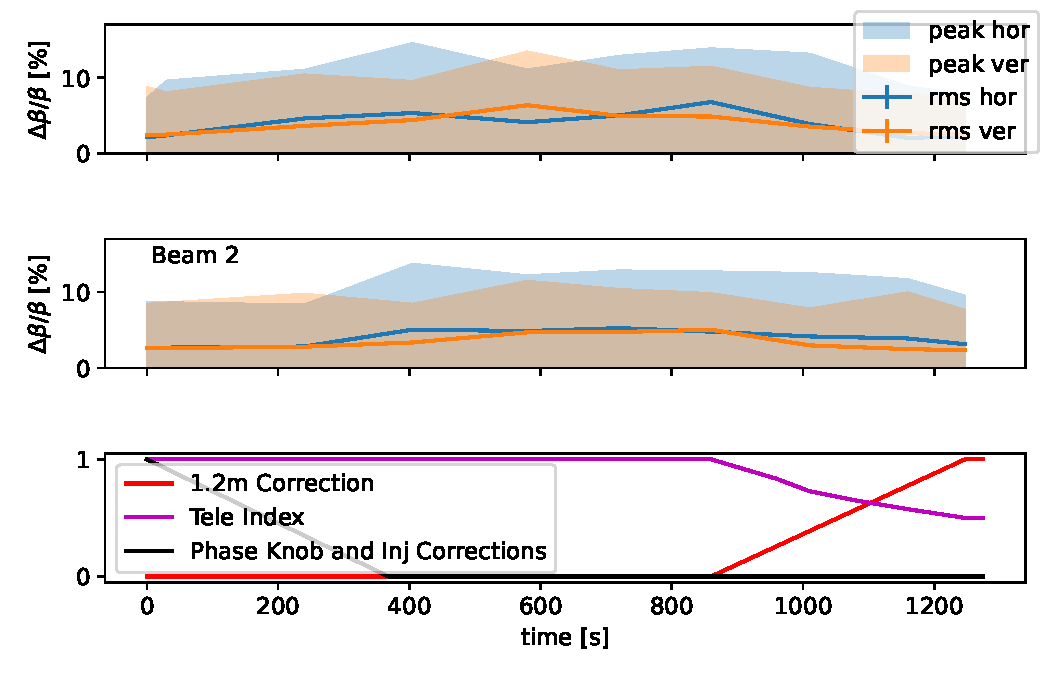
\includegraphics{2023/ramp/rms_in_ramp_with_ats_factor.pdf}
    \caption{The peak and RMS beta-beat along the 2023 ramp after corrections. The lower plot shows how the global corrections at injections are trimmed out as well as the tele-index and how the global corrections are trimmed in towards the end of the ramp. }
    \label{fig:ramp2023_with_all_info}
\end{figure}
\subsubsection{2m}
\begin{figure}[ht]
\begin{subfigure}{.5\textwidth}
  \centering
  % include first image
  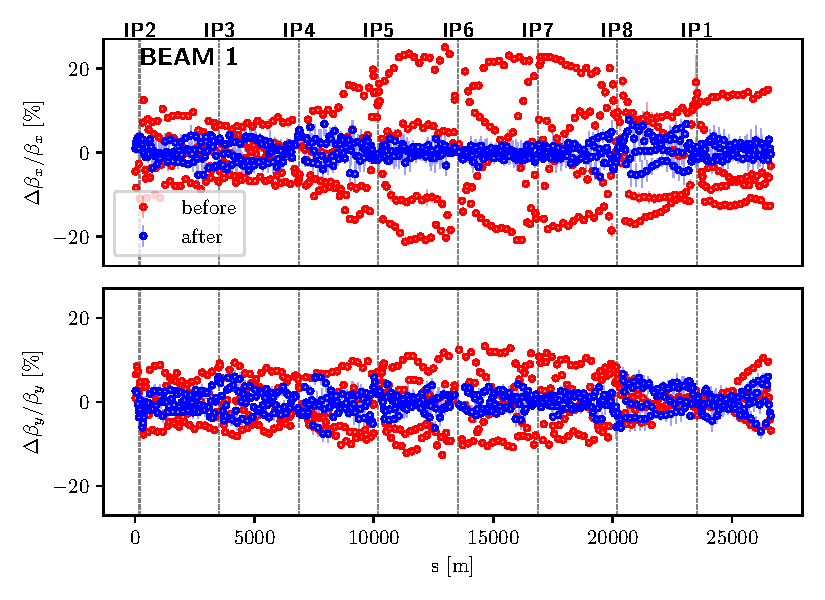
\includegraphics[width=.98\linewidth]{2023/2m/beta_plot_200cm_BEAM_1.pdf}  
  \caption{Beam~1}
\end{subfigure}
\begin{subfigure}{.5\textwidth}
  \centering
  % include second image
  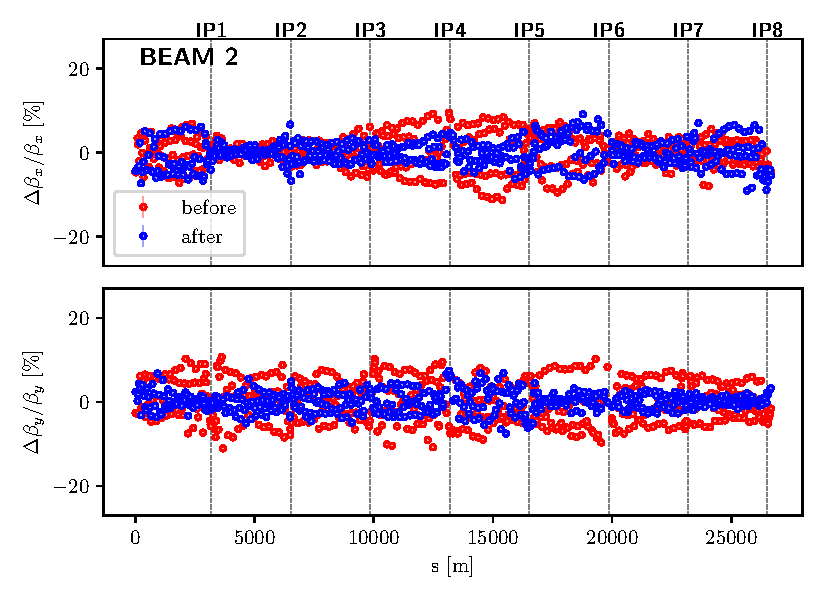
\includegraphics[width=.98\linewidth]{2023/2m/beta_plot_200cm_BEAM_2.pdf}  
  \caption{Beam~2}
\end{subfigure}
\caption{The beta-beat before and after correction. Note that the correction was based on measurement at 1.2~m and then applied at full strength also at 2m. }
\label{fig:2m_before_after_correction}
\end{figure}


\begin{figure}[ht]
\begin{subfigure}{.5\textwidth}
  \centering
  % include first image
  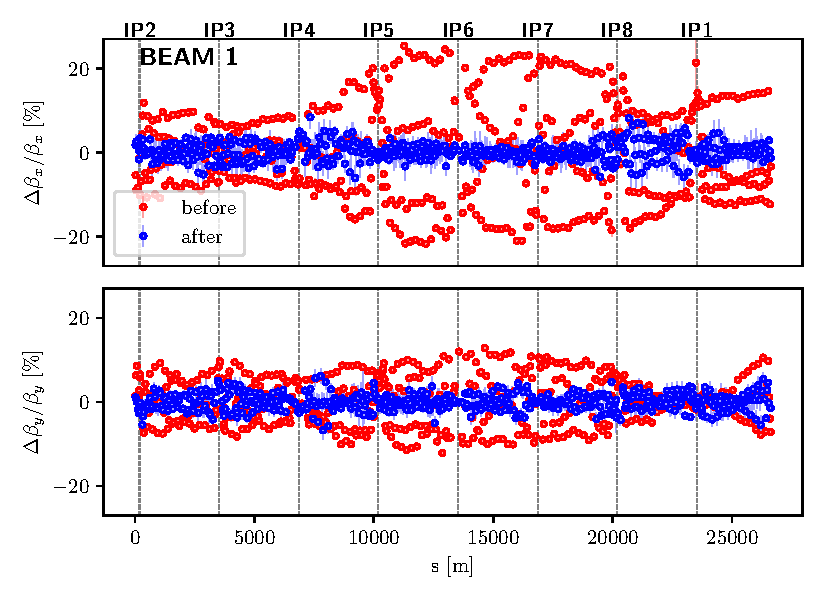
\includegraphics[width=.98\linewidth]{2023/2m/beta_plot_120cm_BEAM_1.pdf}  
  \caption{Beam~1}
\end{subfigure}
\begin{subfigure}{.5\textwidth}
  \centering
  % include second image
  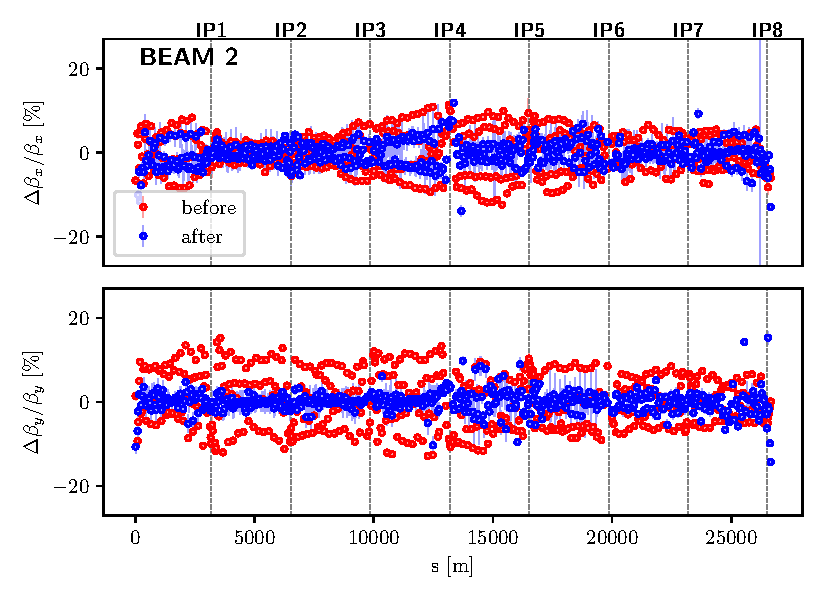
\includegraphics[width=.98\linewidth]{2023/2m/beta_plot_120cm_BEAM_2.pdf}  
  \caption{Beam~2}
\end{subfigure}
\caption{The beta-beat before and after correction at 1.2m.}
\label{fig:2m_before_after_correction}
\end{figure}


\subsubsection{1.2m-30cm}


%knobs name & In $\beta*$ (energy) & Max $\beta*$ (energy) & Out $\beta*$ (energy)

\section{References}
\begin{thebibliography}{99} % Use for 1-9 references

%\bibitem{PhysRevSTAB.15.091001} R. Tom\'as, {\it et al.}, ``Record low $\ensuremath{\beta}$ beating in the LHC''
%Phys. Rev. ST Accel. Beams {\bf 15}, 091001, September 2012.
%\url{https://doi.org/10.1103/PhysRevSTAB.15.091001}

\bibitem{roderik} R. Bruce, {\it et al.}, ``New IR7 optics with removed MQW magnets'',  \href{https://indico.cern.ch/event/681507/contributions/2814548/attachments/1570845/2478033/2017.12.06--HSS_meeting_MQW_removal.pdf}{ABP-HSS Section meetings
Wednesday 6 Dec. 2017}.

\bibitem{ACcom} T.~Persson, {\it et al.}, ``LHC optics commissioning: A journey towards 1$\%$ optics control'', Phys. Rev. Accel. Beams, \textbf{20}, 061002 (2017).
\url{https://doi.org/10.1103/PhysRevAccelBeams.20.061002}

\bibitem{ewen2019jour} E.H. Maclean, {\it et al.}, ``A new approach to the LHC optics commissioning for the nonlinear era'', {\it Phys. Rev. Accel. Beams}  {\bf 22}, p. 061004 (2019).\vspace{-0.03cm}
\url{https://doi.org/10.1103/PhysRevAccelBeams.22.061004}

\bibitem{run3} S. Fartoukh, {\it et al.}, 
	``LHC Configuration and Operational Scenario for Run 3'', CERN-ACC-2021-0007.
	
\bibitem{ats_stephane}
S.~Fartoukh, ``Achromatic telescopic squeezing scheme and its application to the LHC and its luminosity upgrade'', Phys. Rev. ST Accel. Beams {\bf16}, 111002 (2013)

\bibitem{first} M. Aiba, S. Fartoukh, A. Franchi, M. Giovannozzi, V. Kain, M. Lamont, R. Tom\'as, G. Vanbavinckhove, J. Wenninger, F. Zimmermann, R. Calaga, and A. Morita, ``First beta-beating measurement and optics analysis for the CERN Large Hadron Collider'', Phys. Rev. ST Accel. Beams {\bf12}, 081002 (2009).


\bibitem{tomasCERNLargeHadron2010}
R. Tomás, {\it et al.}, “CERN Large Hadron Collider optics
model, measurements, and corrections”, {\it Phys. Rev. Accel. Beams}  {\bf 13}, p. 121004 (2010).
%
\bibitem{record} R. Tom\'as, {\it et al.}, ``Record low beta beating in the LHC'',
Phys. Rev. ST Accel. Beams {\bf15}, 091001, 2012.
%
\bibitem{felixkmod} F. Carlier and R. Tom\'as, ``Accuracy and feasibility of the $\beta^*$ measurement for LHC and High Luminosity LHC using k-modulation'',
Phys. Rev. Accel. Beams {\bf20}, 011005 (2017).
%

%https://journals.aps.org/prab/pdf/10.1103/PhysRevSTAB.13.121004

\bibitem{jaime_rdt}
J. Coello, R. Tom\'as and M. Hofer, ``New local optics measurements and correction techniques for the LHC and its luminosity upgrade'', Phys. Rev. Accel. Beams {\bf 23}, 041001 (2020).
\url{https://doi.org/10.1103/PhysRevAccelBeams.23.041001}

\bibitem{cardona17} J. F.  Cardona, A. C. Garc\'ia, and R. Tom\'as, ``Local correction of quadrupole errors at LHC interaction regions using action and phase jump analysis on turn-by-turn beam position data'', {\it Phys. Rev. Accel. Beams} {\bf 20}, p. 111004 (2017).
\url{https://doi.org/10.1103/PhysRevAccelBeams.20.111004}

\bibitem{cardona20} J. F.  Cardona, Y. Rodr\'iguez, and R. Tom\'as, ``A twelve-quadrupole correction for the interaction regions of high-energy accelerators'',  arXiv:2002.05836 [physics.acc-ph] (2020).

%\cite{Garcia Morales:IPAC21-MOPAB186}
\bibitem{Garcia_Morales:IPAC21-MOPAB186}
   H. Garcia Morales, {\it et al.},
   \textquotedblleft{Comparison of Segment-by-Segment and Action-Phase-Jump Techniques in the Calculation of IR Local Corrections in LHC}\textquotedblright,
   in \emph{Proc. IPAC’21}, Campinas, Brazil, May 2021, pp. 632--635.
   \url{doi:10.18429/JACoW-IPAC2021-MOPAB186}  

\bibitem{ipac2022_apj} J. F. Cardona, {\it et al.}, ``Progress on the action and phase jump for LHC local optics correction'', this conference.


\bibitem{IPAC2020Fol}  E. Fol, {\it et al.},
   \textquotedblleft{Machine Learning Techniques for Optics Measurements and Corrections}\textquotedblright,
   in \emph{Proc. IPAC’20}, Caen, France, May 2020, pp. 61.
   \url{doi:10.18429/JACoW-IPAC2020-WEVIR12} 

\bibitem{epj_efol} E.~Fol, R.~Tom\'as,  G.~Franchetti. ``Supervised learning-based reconstruction of magnet errors in circular accelerators'', Eur.~Phys.~J.~Plus 136, 365 (2021). \url{doi.org/10.1140/epjp/s13360-021-01348-5}

\bibitem{efol_mlcorr_this_conference} E.~Fol, {\it et al.}, ``Experimental Demonstration of Machine Learning Application in LHC Optics Commissioning'', this conference.


\bibitem{evian_2015_langer} A. Langner, {\it et al.}, “Optics model”, Proceedings of the 6th Evian Workshop,
Evian, France, (2015) \url{https://indico.cern.ch/event/434129/contributions/1917199/attachments/1223733/1790347/EVIAN_alangner.pdf}
%
\bibitem{tobias_evian19}
T.~Persson, {\it et al.}, ``LHC Optics Corrections in Run 2, LHC operation Workshop Evian Workshop 2019, Evian France.
\url{https://indico.cern.ch/event/751857/contributions/3259376/attachments/1781875/3033022/optics_corrections_run2.pdf}
%
\bibitem{felix_soubelet_local_coupling_this_conference} F.~Soubelet, {\it et al.}, ``First Interaction Region Local Coupling Corrections in the LHC Run~3'', this conference.
%
\bibitem{michaelcoup} M. Hofer and R. Tom\'as, ``Effect of local linear coupling on linear and nonlinear observables in circular accelerators'',
Phys. Rev. Accel. Beams {\bf23}, 094001, 2020.
%
\bibitem{MDlocalcoupling} T.~Persson, {\it et al.}, ``MD4944: Local linear coupling measurement at the IPs'', CERN-ACC-NOTE-2020-0013.

%\cite{Soubelet:IPAC21-MOPAB007}
\bibitem{Soubelet:IPAC21-MOPAB007}
   F. Soubelet,  {\it et al.} ,
   \textquotedblleft{Prospect for Interaction Region Local Coupling Correction in the LHC Run 3}\textquotedblright,
   in \emph{Proc. IPAC’21}, Campinas, Brazil, May 2021, pp. 61--64.
   \url{doi:10.18429/JACoW-IPAC2021-MOPAB007}  

\bibitem{coup_improved_tpersson} T. Persson and R. Tom\'as, ``Improved control of the betatron coupling in the Large Hadron Collider'',
{\it Phys. Rev. ST Accel. Beams} {\bf 17}, p. 051004 (2014).
\url{https://doi.org/10.1103/PhysRevSTAB.17.051004}
%
\bibitem{ipac2018_automatic_coupling}    T. Persson \emph{et al.},
   \textquotedblleft{Transverse Coupling Measurements With High Intensity Beams Using Driven Oscillations}\textquotedblright,
   in \emph{Proc. IPAC’18}, Vancouver, Canada, Apr.-May 2018, pp. 208--211.
   \url{doi:10.18429/JACoW-IPAC2018-MOPMF047}    
%
\bibitem{josch} J. Dilly, {\it et al.}, ``Controlling Landau damping via feed-down from high-order correctors in the LHC and HL-LHC'', IPAC 2022, this conference.

%\bibitem{jaime_imroved_src} J.M. Coello de Portugal, {\it et al.}, \textquotedblleft{OMC Software Improvements in 2014}\textquotedblright, in \emph{Proc. 6th Int. Particle IPAC'15}, Richmond, VA, USA, May 2015, pp. 426--429. \url{doi:10.18429/JACoW-IPAC2015-MOPJE056}            \vspace{-0.05cm}
%
%\bibitem{p_omc_software19} R. Tom\'as, {\it et al.}, ``LHC Optics Measurement and Correction Software Progress and Plans'', in \emph{Proc. 10th Int. Particle IPAC'19}, Melbourne, Australia, May 2019, paper MOPMP033.

%\bibitem{LSA} G. Kruk, {\it et al.}, ``LHC Software Architecture (LSA) – Evolution towards LHC beam commissioning'', in {\it Proc.} ICALEPCS'07, Knoxville, Tennessee, USA, pp. 307-309.

%\bibitem{nature_NumPy} C.R. Harris, {\it et al.} ``Array programming with NumPy`` Nature 585, 357–362 (2020). \url{https://doi.org/10.1038/s41586-020-2649-2}
%

%\bibitem{lukas_omc_software_ipac} L.~Malina, {\it et al.}, ``Analysis framework of beam optics measurements and corrections in synchrotrons'', this conference.
%\bibitem{lukas_omc_software_ipac} L.~Malina, {\it et al.}, ``OMC3'', \url{https://github.com/pylhc/omc3}

%\bibitem{Harpy} L.~Malina, ``Harpy: A fast, simple and accurate harmonic analysis with error propagation'', this conference.
%\bibitem{Harpy} L.~Malina, ``Harpy'', \url{https://github.com/pylhc/omc3/tree/master/omc3/harpy}


%\bibitem{sussix} R. Bartolini and F. Schmidt, ``Sussix: A computer code for
%frequency analysis of non–linear betatron motion'', CERNSL-Note-98-017, 1998.

%\bibitem{IF_prab} E. Fol {\it et al.}, ``Detection of faulty beam position monitors using unsupervised learning'', \textit{Phys. Rev. Accel. Beams} {\bf 23}, p. 102805 (2020).
%\url{https://doi.org/10.1103/PhysRevAccelBeams.23.102805}
   %

%\bibitem{efol_denoising_ipac_2021} E.~Fol, and R.~Tom\'as, ``Denoising of optics measurements using Autoencoder Neural Networks'', this conference.

%\bibitem{efol_ml_optics_ipac_2021} E.~Fol, H.~Garcia Morales and R.~Tom\'as, ``Reconstruction of linear optics observables using supervised learning, this conference.

 

%\bibitem{hector_tune_cleaning} H.~G.~Morales, R.~Tom\'as, ``Unsupervised learning techniques for tune cleaning measurement'', this conference.

%\bibitem{hector20} {H. Garcia-Morales et al., "Phase advance constraint in K-modulation for $\beta^\ast$ determination in the LHC", Submitted to PRAB (2020)}.

%\bibitem{ana_prab_calib} A. Garc\'ia-Tabar\'es Valdivieso and R. Tom\'as,  ``Optics-measurement-based beam position monitor calibrations in the LHC insertion regions'', Phys. Rev. Accel. Beams {\bf 23}, 042801 (2020).
%\url{https://doi.org/10.1103/PhysRevAccelBeams.23.042801}

%\bibitem{jaqueline_ipac2021_compac} J. Keintzel, {\it et al.}, ``Momentum compaction factor measurements for the Large Hadron Collider'', this conference. 


%\bibitem{andreas_coupling_ipac} A. Wegscheider and R.~Tomas, ``Forced coupling Resonance Driving Terms'', this conference.

%\bibitem{adt_coupling_online} A.~Calia, {\it et al.}, ``Online coupling measurement and correction throughout the LHC Cycle'', in \emph{Proc. ICALEPCS'17}, Barcelona, Spain, October 2017, paper TUPHA119, pp. 686-691.

%\bibitem{rtomas_opti_coupling_knobs} R.~Tom\'as, ``Optimizing the global coupling knobs for the LHC'', CERN-ATS-Note-2012-019 MD.
%

%\bibitem{eirik_ipac} E.~J~H{\o}ydalsvik and T.~Persson, ``Reaching the sub per mil level coupling corrections in the LHC'', this conference.

%\bibitem{mcs_md_report} T.~Persson, {\it et al.}, ``LHC 3324: Counteracting coupling decay at injection'', CERN-ACC-NOTE-2021-0008.

%\bibitem{FelixRDTpaper} {F.S.~Carlier}, {R.~Tom\'as} and {E.H.~Maclean}.
%\newblock {Measurement and Correction of Resonance Driving Terms in the Large Hadron Collider}, Submitted to Phys.~Rev.~Accel.~Beams.


\end{thebibliography}


\end{document}